%
% TeX template for Master Thesis of Tohoku University
%
% (English thesis)
%
\documentclass[12pt]{article}

\usepackage{url}
\usepackage{graphicx}
\usepackage{multirow}
\usepackage{tabularx}
\usepackage{longtable}
\usepackage{enumerate}

\usepackage{pdfpages}
\usepackage{rotating}
\usepackage{subcaption}
\usepackage{hyperref}


\usepackage[english]{babel}
\usepackage{xeCJK}
\setCJKmainfont{MS Mincho} % for \rmfamily
\setCJKsansfont{MS Gothic} % for \sffamily

\usepackage{amsmath}
\usepackage{algorithm}
\usepackage[noend]{algpseudocode}
\makeatletter
\def\BState{\State\hskip-\ALG@thistlm}
\makeatother

\setlength{\topmargin}{0.5cm}
\setlength{\textheight}{20.5cm}
\setlength{\textwidth}{14.5cm}
\setlength{\oddsidemargin}{0.6cm}
\setlength{\evensidemargin}{-3.8cm}
\setlength{\parindent}{1em}
\renewcommand{\baselinestretch}{1.2}

\begin{document}

%\includepdf{yobishinsaCover.pdf}

% Language Selection
% For English
\input tohoku-mthesis.sty
% For Japanese
%\input tohoku-jmthesis.sty

% Student Number
\studentnumber{B5IM2034}

\doctitle{\mastersthesis}
\major{\information}

% Title in Japanese
%\title{}
% Title in English
\etitle{Semantic parsing with a domain ontology\\
領域オントロジーを用いた\\
セマンティックパージング}

% Author name in Japanese
%\author{いぬたろう}
% Author name in English
\eauthor{Corentin DUMONT}

% Submission date
\syear{2017}
\smonth{3}
\sday{24}

% committee members
% Supervisor, Co-supervisor, and Member must be specified.
% For Japanese
%\cmembers{乾 健太郎 教授}{(主指導教員)}
%         {○○ ○○ 教授}{(副指導教員)}
%         {○○ ○○ 准教授}{(副指導教員)}
%         {○○ ○○ 准教授}{(△△大学)}
% For English
\ecmembers{Professor Kentaro Inui}{(Supervisor)}
          {Professor Yoshifumi Kitamura}{}
          {Professor Tetsuo Kinoshita}{}
          {Associate Professor Naoaki Okazaki}{(Co-supervisor)}

% keywords in Japanese
%\keywords{}
% keywords in English
\ekeywords{Knowledge acquisition, Ontology, Semantic parsing, Question Answering}

% Abstract in Japanese
%\abstract{}
% Abstract in English
\eabstract{
Using restricted domains in question answering (QA) allows to build an ontology of the domain that can be used with by a semantic parser to improve the performance of a QA system. However, building an ontology and a semantic parser can be costly and usually require a large amount of annotated data that may not be available for specific domains. Our work is a case study on how to build a semantic parser and a domain ontology with very low resource for the video game Minecraft.\\
%We present a collection of data about the Minecraft domain, which includes a knowledge corpus and a domain ontology, and the creation and training results of a semantic parser for Minecraft that uses the domain ontology. We also suggest some guidelines for reflection on how to use our semantic parser to do question answering in Minecraft.\\
%The game Minecraft has been chosen for its popularity among players that ensure that written knowledge about it can be collected from the web, and for its popularity among researchers from several artificial intelligence (AI) domains that could give more impact to our work.\\
We show that the creation of a semantic parser and the ontology it is based on can be done with a very low amount of expert manual annotations, facilitated by the use of automatically collected data from the web, and that fairly good performance can be obtained.
%Furthermore, we show that it is possible to increase the size of the annotated data even with non-expert annotations done with crowd-sourcing.\\
Thus, as a contribution, this case study is a first step in solving the common problem of building a QA system in a restricted domain from very low resource and low manual effort.
}

%%%%%%%%%%%%%%%%%%%%%%%%% document starts here %%%%%%%%%%%%%%%%%%%%%%%%%%%%

% cover page and abstract
\titlepage
\cmemberspage
\firstabstract
\newpage

% table of contents
\tableofcontents
\newpage
\listoffigures
\newpage
\listoftables
\newpage
\pagenumbering{arabic}

% main texts

\section{Introduction}
The initial motivation of this work is to improve the interaction between the players and Non-Player Characters (NPCs) in video games.
As in Figure~\ref{currentInteraction}, in current video games, interaction between the player and the NPCs is very limited in the sense that the player cannot ask his own questions.
Indeed, the game will often propose several possible questions or choices to the player, who can only choose among them.\\
\begin{figure}[!ht]
	\centering 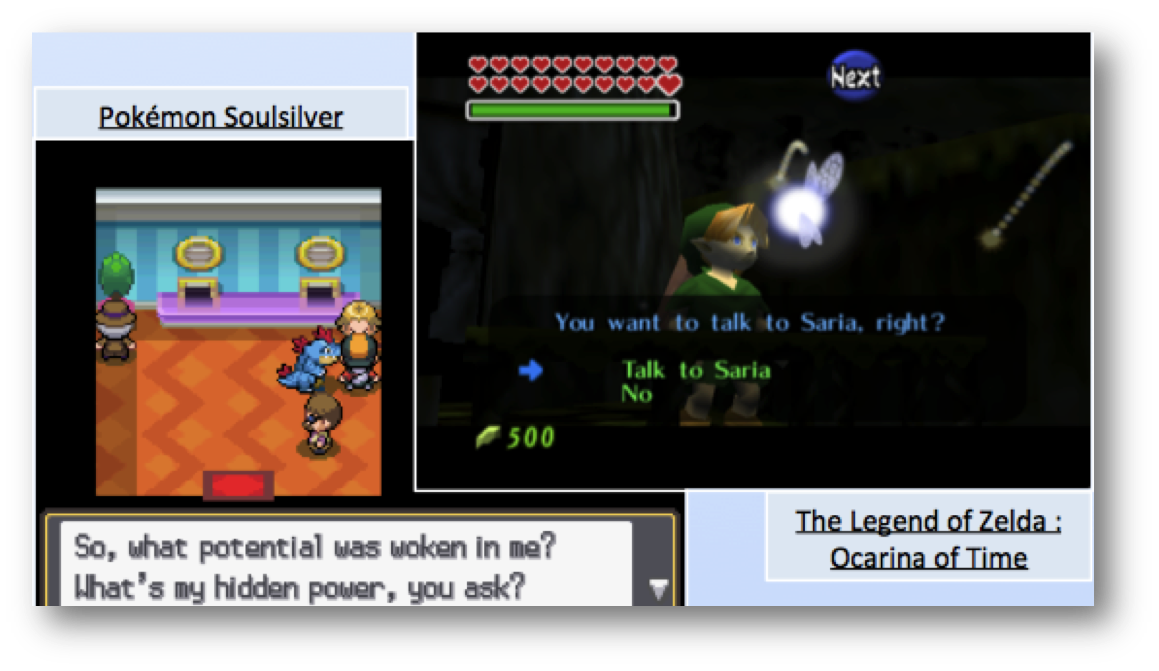
\includegraphics[width=0.9\linewidth]{Figures/Intro_Conclusion/currentInteraction.png}
	\caption{\label{currentInteraction}Interaction between players and NPCs in current video games}
\end{figure}
Our final goal is to develop a natural language question answering system that would make possible a real interaction between the player and the NPCs.
Such a system, as shown in Figure~\ref{goal}, would allow the player to ask about anything in English about the content of the game, and make the NPCs able to answer in natural English to any question of the player as long as it is about the content of the game.\\
\begin{figure}[!ht]
	\centering 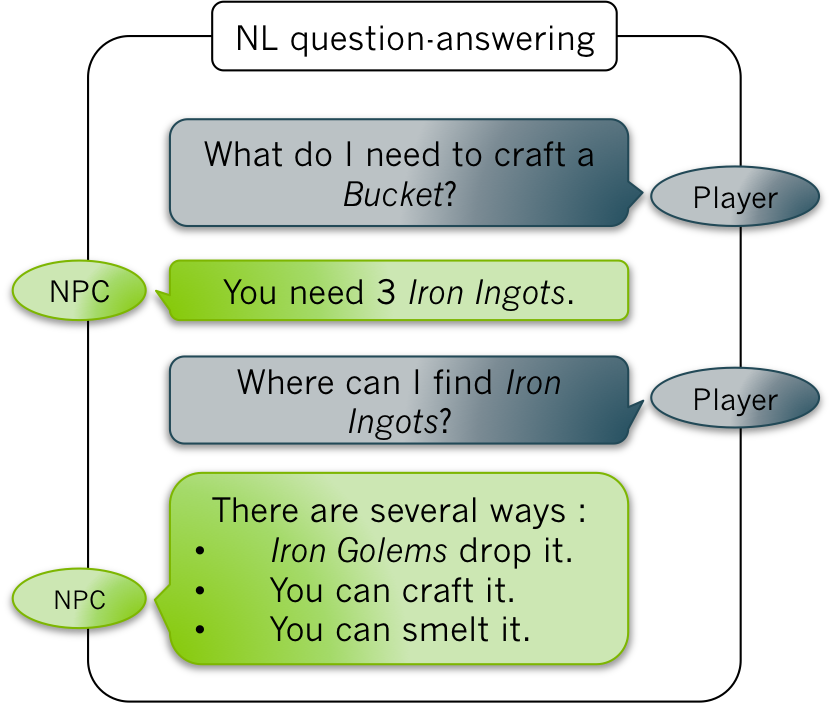
\includegraphics[width=0.7\linewidth]{Figures/Intro_Conclusion/goal.png}
	\caption{\label{goal}The final goal of our work, a natural language QA system}
\end{figure}
Unlike many QA systems that are designed to answer real world questions \cite{berant2014semantic,yao2015lean}, the final goal of this research is to build a system that can answer questions using the logic specific to the game, which may not be identical to the logic in the real world. For our study, we choose a popular game called Minecraft, whose openness provides a great liberty for players, which guarantees a large number of possible questions to ask about the game, and yet the presence of a specific logic that limits the actions of players. We are interested in this problem setting because it provides a testbed for combining Natural Language Processing with advanced logical inference techniques.\\
Our final system should be able to access knowledge about the content of the game, so we need to collect this knowledge.
It should also understand the content of this knowledge and the players' questions in order to construct a relevant answer, so we need to build a semantic parser that will extract the meaning from English sentences by finding the important instances and the relations that link these instances together.
Finally, it has to answer the questions by constructing relevant answers from the knowledge it has about the game using logical inference techniques.\\
As a whole, our work is a case study on how to build a Semantic Parser (and in the end, a complete Question Answering system) from very low resource in the restricted domain of a video game.

\newpage
\section{Case study: Minecraft}

\subsection{Minecraft}

\begin{figure}[!ht]
	\centering 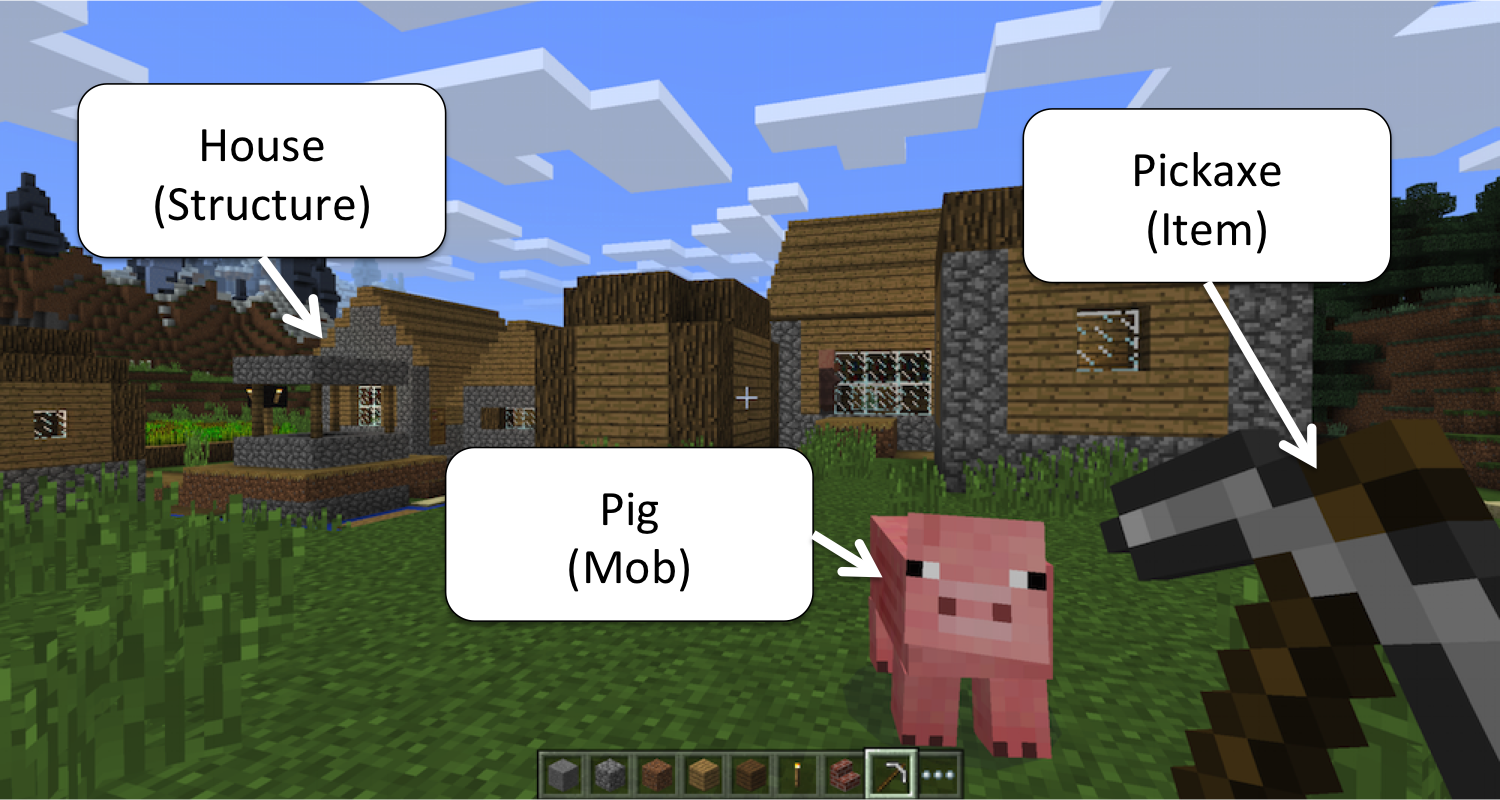
\includegraphics[width=0.7\linewidth]{Figures/Minecraft/minecraft.png}
	\caption{\label{minecraftPicture}A snapshot of Minecraft}
\end{figure}

\begin{figure}[!ht]
	\centering 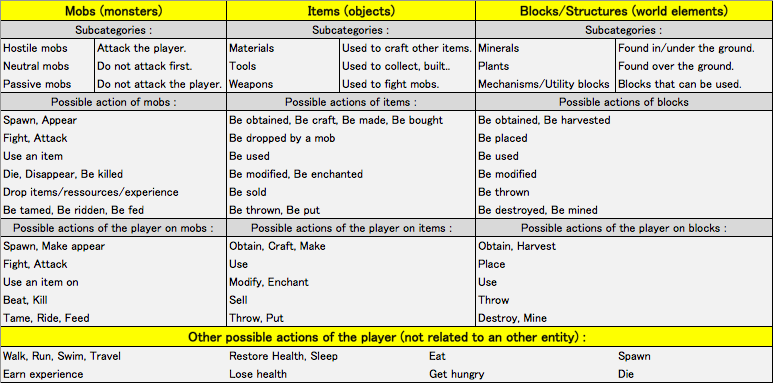
\includegraphics[width=\textwidth]{Figures/Minecraft/tableEntitiesActions.png}
	\caption{\label{minecraftActions}Entity types and actions in Minecraft}
\end{figure}

Minecraft (Figure~\ref{minecraftPicture}) is a sandbox video game, which means that the player is free to choose the actions he wants to execute, and the order of these actions. However, as all video games, the number of possible actions is limited. The main occupation of the player in Minecraft is to survive in a world populated by monsters, by finding resources (e.g. mining minerals, growing plants, etc.), to create structures, items and weapons (i.e. crafting them with the collected resources by following recipes) and beating monsters using crafted weapons and items to protect the created structures and earn experience and new items, in order to continue to develop.\\
The different entities of the game follow a hierarchy. Entities can be divided into Structures, Mobs (monsters), and Objects, which are divided into Items (for example used to fight) and Blocks (used to build Structures), and so on. The player can interact with these entities, or make independent actions. These actions and interactions are summarized in the Figure~\ref{minecraftActions}.\\
Minecraft players usually ask about:\\
properties of entities,
\begin{quote}
\textit{How many health point does a iron golem have?} (100)
\end{quote}
relations between entities,
\begin{quote}
\textit{What is a cake composed of?} (milk, sugar, egg and wheat)
\end{quote}
or conditions and effects of actions.
\begin{quote}
\textit{What pickaxe is needed to break a diamond block?} (iron pickaxe or diamond pickaxe)\\
\textit{How can I get a door?} (craft door, find door in village)
\end{quote}
The knowledge needed to answer most of Minecraft players' questions are available on several websites dedicated to Minecraft that are often written by players themselves.

\subsection{Why Minecraft?}
Why did we choose Minecraft for our case study?\\
The liberty of the player guarantees a large number of possible questions to ask about the game, but the game follows nonetheless a logic that can be learned by a QA system to increase its ability to understand the meaning of the questions.\\
In other words, Minecraft players are likely to ask non-trivial and difficult questions like:
\begin{quote}
\textit{What is the best way to obtain Obsidian?}
\end{quote}
To answer this question, we need to know about all the different ways to obtain \textit{obsidian}, and we need to compare these methods, which is not possible if we do not understand them. However, the strict logic that rules the game makes these difficult questions possible to answer by an automatic QA system, contrary to such questions in the real world. For example, thanks to this strict logic, in the following sentences:
\begin{quote}
\textit{The player kills a wolf with a ???.}
\end{quote}
an automatic system can deduce that ??? can only be replaced with \textit{sword}, \textit{pickaxe}, \textit{axe} or \textit{shovel}. This kind of logic can be used to resolve ambiguities.\\
Our final goal is to build a QA system that can translate a question asked by players to a series of queries about the entities and actions in the game, and find a relevant answer in the knowledge database among all the information about these entities and actions, possibly by combining several pieces of knowledge together to answer difficult questions.\\
Since Minecraft is a popular game, we expect that we can find abundant data from the Web. Furthermore, Minecraft has been the domain for other works on artificial intelligence \cite{branavan2012learning,johnson2016malmo}, and not only in natural language processing (NLP). So choosing Minecraft as a domain can make our work more valuable and have a better impact.\\
There have been many efforts done to restrict the domain of the QA task and pursue some advanced reasoning. The Todai Robot Project \cite{fujita2014overview} restricts the domain to university entrance exam questions. Other research includes solving algebra word problems \cite{kushman2014learning} and instructing robots \cite{misra2015environment}. As a complement to these previous works, we believe the using of an open world video game as the domain has several merits. Firstly, the logic in a video game is simpler than the real world, which means that it can be handled readily. Therefore, this domain may provide a convenient testbed for integrating logical inference techniques into NLP systems, such as the logical inference using dependency-based compositional semantics \cite{tian2014logical}. Secondly, despite the rather simple rules, open world video games provide enough liberty for players, and their popularity attracts people to ask many questions about them, including creative and fun questions that can be solved only by completely understanding the rules and logically combining them. Therefore, we expect the domain to be interesting and challenging as well.

\newpage
\section{Collect data about Minecraft}

\subsection{Knowledge corpus}
A knowledge database is extracted from three different wiki-like websites\footnote{
\href{http://www.minecraft.gamepedia.com/}{www.minecraft.gamepedia.com}
\\\href{http://www.minecraft.wikia.com/}{www.minecraft.wikia.com}
\\\href{http://www.minecraftguides.org/}{www.minecraftguides.org}}. These websites are constituted of pages describing an entity or a concept of the game. Similar to those from Wikipedia, the web-pages can be divided into two parts, namely the structured data such as infoboxes, tables, or web-pages hierarchy, and unstructured data such as natural language texts (Figure~\ref{websites}).

\begin{figure}[!ht]
	\centering 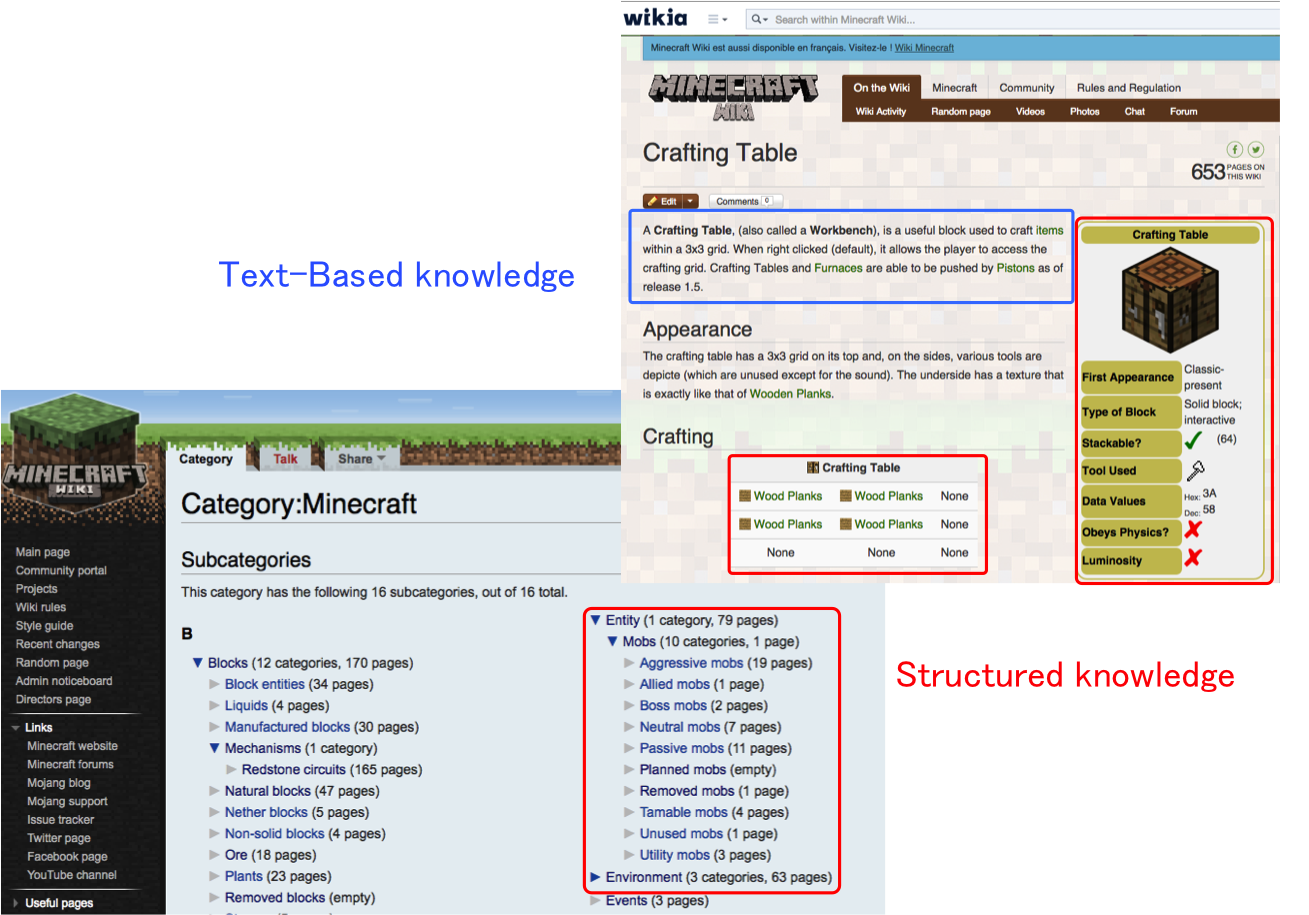
\includegraphics[width=\textwidth]{Figures/Knowledge/websites.png}
	\caption{\label{websites}Text and structured data in the websites used for knowledge extraction}
\end{figure}

We preserve the structures of infoboxes and tables in our extraction, and separate structured and unstructured data. As a result, we obtain a database composed of 1063 unique text files, organized in 51 folders and sub-folders to regroup related objects (see Table~\ref{tableDB} for details).

\begin{sidewaystable}[!htbp]
	\centering
	\begin{tabular}{|c|c|c|c|}
	\hline
	\multicolumn{2}{|c|}{Folders} & Number of Files & Description\\
	\hline
	 & Blocks & 154 & Environment's blocks\\
	\cline{2-4}
	DB-Gamepedia & Entity & 72 & Mobs (Monsters)\\
	\cline{2-4}
	(from minecraft.gamepedia.com) & Items & 161 & Objects used by the player\\
	\cline{2-4}
	 & Others & 183 & Gameplay, History, etc.\\
	\cline{2-4}
	 & \multicolumn{3}{|c|}{Total: 530 files}\\ %$=>$\ Total & 530 & Different files\\
	\hline
	 & Blocks & 200 & \\
	\cline{2-4}
	DB-Wikia & Items & 167 & \\
	\cline{2-4}
	(from minecraft.wikia.com) & Main & 23 & Important objects/entities\\
	\cline{2-4}
	 & Mobs & 56 & \\
	\cline{2-4}
	 & \multicolumn{3}{|c|}{Total: 392 files}\\ %$=>$\ Total & 392 & Different files\\
	 \hline
	 & Blocks & 101 & Minerals, Plants, etc.\\
	\cline{2-4}
	 & Brewing & 34 & Recipes of potions\\
	\cline{2-4}
	 & Building & 7 & \\
	\cline{2-4}
	 & Farming & 7 & \\
	\cline{2-4}
	DB-Guides & Items & 77 & Food, Tools, Weapons, etc.\\
	\cline{2-4}
	(from minecraftguides.org) & Main & 10 & Summaries of sub-folders\\
	\cline{2-4}
	 & Mini-Games & 25 & \\
	\cline{2-4}
	 & Mobs & 27 & \\
	\cline{2-4}
	 & Tutorials & 30 & \\
	\cline{2-4}
	 & \multicolumn{3}{|c|}{Total: 300 files}\\
	\hline
	 \multicolumn{4}{|c|}{Total: 1063 unique files (1222 extracted files)}\\
	\hline
	\end{tabular}
   	\caption{\label{tableDB} A summary of the knowledge database}
\end{sidewaystable}

To improve the quality of the extracted data, we defined extracting rules for each of the 3 websites. The main purpose of these rules is to extract separately structured and unstructured data, to remove useless information and to avoid extracting segments of sentences that loose their meaning out of context (see Figure~\ref{extractingules})

\begin{figure}[!ht]
	\centering 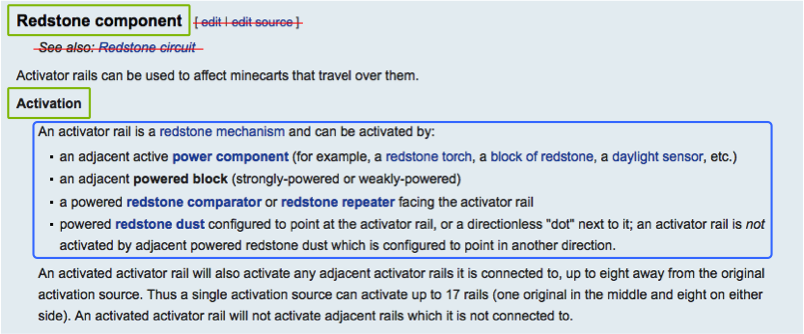
\includegraphics[width=\textwidth]{Figures/Knowledge/extractingRules.png}
	\caption{\label{extractingules}Extraction of Minecraft knowledge from websites}
\end{figure}

\subsection{Question corpus}
A corpus of questions and answers has been created on the basis of posts extracted from quiz websites\footnote{
\href{http://www.quizlet.com/}{www.quizlet.com} 
\\\href{http://www.allthetests.com/}{www.allthetests.com} 
\\\href{http://www.gamefaqs.com/}{www.gamefaqs.com}}. 754 questions have been collected from different websites, and 544 of them have been extracted with their answer.\\
Then, we manually selected 100 relevant questions. For our purpose, it is important that the questions deal with facts inside the game, and not facts that are outside the game (e.g. questions about the creator of the game, the programming language used, etc.).

\begin{table}[!ht]
\center
\begin{tabular}{|l|}
\hline
\textbf{Factoid questions:}\\
\hline
\textit{What Item should I use to tame a Wolf?}\\
\hline
\textit{Are Spiders Hostile?}\\
\hline
\\
\hline
\textbf{Non-factoid questions:}\\
\hline
\textit{What is the best way to spawn the two}\\
\textit{different types of Golem?}\\
\hline
\textit{Is it interesting to kill the Ender Dragon?}\\
\hline
\end{tabular}
\caption{\label{tableFactoidNonfactoid} Example of factoid and non-factoid questions}
\end{table}

We selected both factoid and non-factoid questions (see Table~\ref{tableFactoidNonfactoid}), and tried to include as much language variety (vocabulary and grammar) as possible in the reference to the concepts of the game. For each selected question, we wrote about nine questions with the same meaning but asked differently, or with a close or related meaning (Table~\ref{tableSimilarQuestions}).

\begin{table}[!ht]
\center
\begin{tabular}{|c|l|}
\hline
0 & \textit{Where do you find a Mushroom?}\\
\hline
1 & \textit{How do you obtain a Mushroom?}\\
\hline
2 & \textit{How do I get a Mushroom?}\\
\hline
3 & \textit{Where can I get a Mushroom?}\\
\hline
4 & \textit{Where can I obtain a Mushroom?}\\
\hline
5 & \textit{What is a way to get a Mushroom?}\\
\hline
6 & \textit{How to get Mushrooms?}\\
\hline
7 & \textit{Where do I find Mushrooms?}\\
\hline
8 & \textit{Where are Mushrooms located?}\\
\hline
9 & \textit{Where can Mushrooms be found?}\\
\hline
\end{tabular}
\caption{\label{tableSimilarQuestions} Examples of similar questions written}
\end{table}

This way, we obtained a corpus that can be used for handling language variations in the QA task. We finally obtained a corpus of 1684 questions, among which 928 has been written on the basis of 100 relevant questions.

\subsubsection{Can the questions be answered by the knowledge corpus?}

From the questions that have been extracted from quizzes websites, we can distinguish 3 types of questions. Some questions are not relevant, because they deal with some facts external to the game itself, or because they contain a mistake:
\begin{quote}
\textit{What is the name of the famous yellow duck who plays Minecraft on YouTube?} (YouTube is external to the game.)\\
\textit{What are the 5 types of wood?} (There are actually 6 types of wood.)
\end{quote}
Some questions can be ``easily'' answered with the knowledge database. This is the case when the answer is clearly written in the database (for example a numeric value in a table). The questions that can be ``easily'' answered are often factoid questions:
\begin{quote}
\textit{How many hearts does a Giant have?} (The answer, 50 hearts, is written in the infobox of the Giant.)
\end{quote}
This kind of question can be answered simply by locating the place where the answer is written in the database. However, some questions can be answered only by computing the answer using crossed information. This is the case of non-factoid questions, which can be considered as ``difficult'' to answer:
\begin{quote}
\textit{What is the best strategy for finding diamonds?} (To answer this question, the system has to find all the different ways to find diamonds and evaluate the efficiency of each method. This evaluation is challenging because the criteria for a good strategy are not stated in the question.)
\end{quote}
In our data, the non-relevant questions are rare (about 2\%), whereas the non-factoid questions are quite common (about 20\%), which provides a good motivation for a QA system to handle complicated questions.\\
However, answering non-factoid questions implies reasoning, i.e. logic inference on different pieces of information contained in the knowledge database, which can only be done on a structured database. This is why we defined the ontology of a meaning representation, which is used to structure the natural sentences of the database to their logical form. The challenge is to balance the complexity of the meaning representation, as it must be simple to take advantage of the simple logic of the game, but must be expressive enough so that it can be used to structure all the useful information.

\subsection{Minecraft Ontology}
Our ontology defines two types of classes to represent the instances in Minecraft and the relations that links these instances together.\\

The \textbf{Instance classes} regroup Minecraft Entities and Events (Figure~\ref{entitiesAndEvents}).

\begin{figure}[!ht]
   \centering 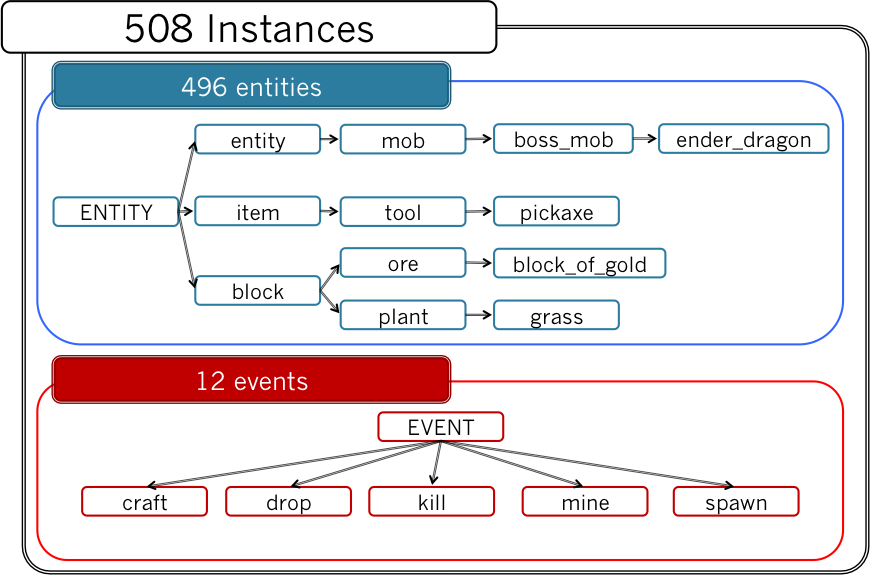
\includegraphics[width=0.7\linewidth]{Figures/Knowledge/entitiesAndEvents.png}
   \caption{\label{entitiesAndEvents} Instances of the Ontology}
\end{figure}

Entity classes include all Structures, Objects (e.g. Blocks, Items, \emph{etc.}) and Mobs that the player can interact with. The ontology defines the list of 496 Entities and their hierarchy (e.g. the Minecraft Entity ``\emph{Stone}'' is a subclass of ``\emph{Natural Block}''). The list of entities and their hierarchy is constructed by checking named entities appeared in our QA corpus and using the hierarchy of web-pages of the Gamepedia website. This list is supposed to have high coverage. We have regrouped some concepts that are usually used by players as different ones but are actually the same objects in the game. For example, both ``\textit{chicken}'' and ``\textit{chick}'' are represented by the same Minecraft Entity class \textit{Chicken}, and are considered as two variations of this class. The regrouping is done because these entities have similar interactions with the player and other entities, and has been mainly done automatically by using the infoboxes of the Gamepedia website that lists the possible variations of entities.\\
Event classes are used to represent events or actions in the game. We make the list of Event classes by considering possible operations by the player and checking questions asked in our QA corpus. We tried to minimize the number of Event classes by regrouping some events that can be expressed as the same actions linked to different Minecraft Entities. For example, both the actions \textit{sleep} and \textit{eat} are regrouped into the event \textit{use}, because ``\textit{sleeping}'' and ``\textit{eating}'' are equivalent to ``\textit{using}'' the Minecraft Entities \textit{bed} and \textit{food}, respectively. There is currently no hierarchy between event classes, except a common root EVENT class, but the fact that entities and events are regrouped under instance classes and used similarly by our classification models would make very easy to add an event hierarchy in the ontology.\\
Besides the hierarchy, each instance class is further defined in the ontology (example in Figure~\ref{exampleEntity}).\\

\begin{figure}[!ht]
   \centering 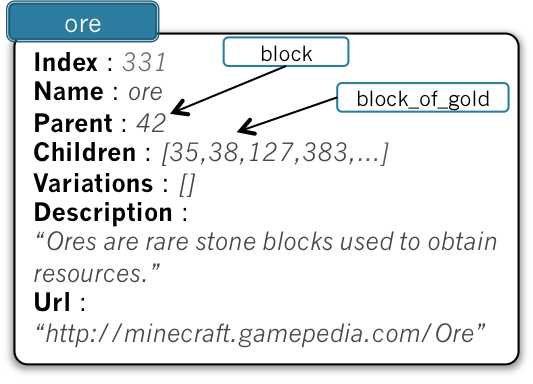
\includegraphics[width=0.6\linewidth]{Figures/Knowledge/exampleEntity.png}
   \caption{\label{exampleEntity} Example of instance: Ore (entity)}
\end{figure}

The \textbf{Relation classes} represent a link between two instances. The ontology defines the list of 54 relation classes and the constraints that define what instances classes can be linked using each relation class. Relation classes are divided in assertion relations (or factual relations, we will use ``\_'' at the beginning of the name) and non-assertion relations (see Figure~\ref{relations}). While assertion relations are used to express a piece of information (e.g. property of an instance, or causality link between to events), non-assertion relations are used to express the semantic link between two instances that appear in the same piece of information (e.g. in the sentence ``The player can kill a wolf with a golden sword'', the ``golden sword'' is the weapon used to ``kill'', so the event ``kill'' is linked to the entity ``golden sword'' by the relation ``weapon''.)

\begin{figure}[!ht]
   \centering 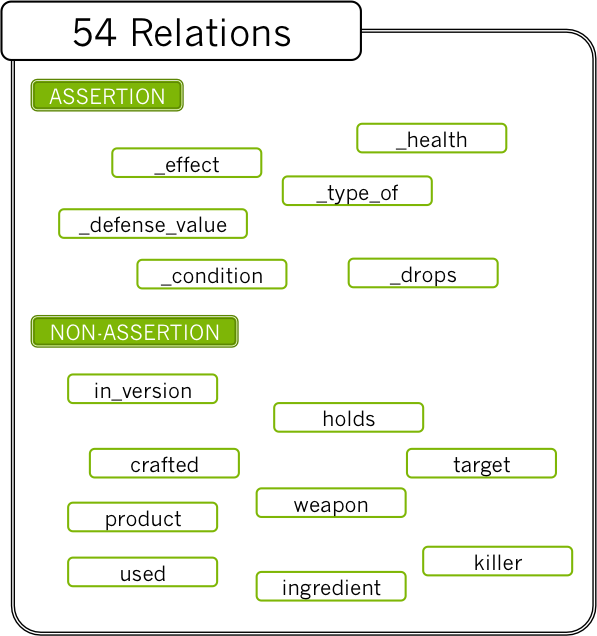
\includegraphics[width=0.5\linewidth]{Figures/Knowledge/relations.png}
   \caption{\label{relations} Relations of the Ontology}
\end{figure}

Each relation class is further defined in the ontology (example in Figure~\ref{exampleRelation}).

\begin{figure}[!ht]
   \centering 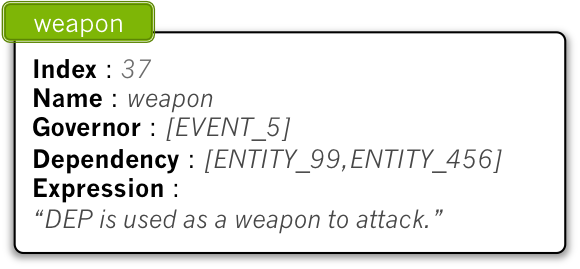
\includegraphics[width=0.6\linewidth]{Figures/Knowledge/exampleRelation.png}
   \caption{\label{exampleRelation} Example of relation: Weapon (non-assertion)}
\end{figure}

We can use a Davidsonian style representation to write knowledge with our ontology. Instances are then associated to a variable name (e for events, x for entities) and Relations are represented by predicates on these variables. For example, an entity $x_1$ dropping an item $x_2$ is represented as 
\begin{quote}
$drop(e), dropper(e, x_1), dropped(e, x_2)$.
\end{quote} 

A piece of information can be asserted by a assertion relation of our ontology, but the existence of a set of instances linked by non-assertion relation in the knowledge database also represents a piece of information. In other words, there are two types of facts. The first type regards the relation between two instances (entities or events), such as a comparison, a subsumption, or a causal relation (effect or condition), expressed by an assertion relation (Figure~\ref{fact1} or Figure~\ref{fact2}). The second type describes a single Minecraft Instance in the game by linking it with other instances through non-assertion relations and express for example the properties of an entity or the probability of an event to occur  (Figure~\ref{fact3}).

\begin{table}[!ht]
\center
\begin{tabular}{|c|}
\hline
\textit{Gold is a type of ore.}\\
\hline
\textit{$gold(x_1), ore(x_2)$}\\
\\
\textit{$\_type\_of(x_1,x_2)$}\\
\hline
\end{tabular}
\caption{\label{fact1} A fact (the first type) representing a subsumption between entity classes.}
\end{table}

\begin{table}[!ht]
\center
\begin{tabular}{|c|}
\hline
\textit{If a chicken dies while on fire, it drops cooked}\\
\textit{chicken instead of raw chicken.}\\
\hline
\textit{$chicken(x_1), kill(e_1), fire(x_2), drop(e_2),$}\\
\textit{$cooked\_chicken(x_3), raw\_chicken(x_4),$}\\
\\
\textit{$killed(e_1,x_1), weapon(e_1,x_2),$}\\
\textit{$dropper(e_2,x_1), dropped(e_2,x_3),$}\\
\\
\textit{$\_effect(e1,e2)$}\\
\hline
\end{tabular}
\caption{\label{fact2} A fact (the first type) about causality between events.}
\end{table}

\begin{table}[!ht]
\center
\begin{tabular}{|c|}
\hline
\textit{Stone can be mined with a pickaxe.}\\
\hline
\textit{$stone(x_1), mine(e_1), pickaxe(x_2)$}\\
\\
\textit{$mined(e_1,x_1), tool(e_1,x_2)$}\\
\hline
\end{tabular}
\begin{tabular}{|c|}
\hline
\textit{Bats usually spawn in caves.}\\
\hline
\textit{$bat(x_1), spawn(e_1), cavern(x_2),$}\\
\\
\textit{$spawned(e_1,x_1), in\_environment(e_1,x_2),$}\\
\hline
\end{tabular}
\caption{\label{fact3} Facts (the second type) on properties of single events.}
\end{table}

As an example of possible logical inference, the following piece of information is written in our knowledge database: 
\begin{quote}
\textit{If a chicken dies while on fire, it will drop cooked chicken.}
\end{quote}
Then, assuming the system has the following common sense knowledge (axiom): 
\begin{quote}
\textit{If an item is dropped, the player gets it.}
\end{quote}
we can deduce the following: 
\begin{quote}
\textit{If a chicken is killed by fire, the player gets cooked chicken.}
\end{quote}
A system equipped with logical inference ability can thus answer a question such as:
\begin{quote}
\textit{How to obtain cooked chicken?}
\end{quote}
by the inference process described above and responds: 
\begin{quote}
\textit{You should kill a chicken with fire.}
\end{quote}

\subsubsection{Can our meaning representation express enough information?}

A question will be answerable if the answer is present in the knowledge database (the question is theoretically answerable), and if all the pieces of information that are needed to answer can be represented with our meaning representation. We expect the contents extracted from the 3 complete websites to have a high coverage, so most of the relevant questions are theoretically answerable. The quality of our QA system will then directly depend on the quantity of relevant pieces of information (that can be used to answer players' questions) that can be represented with the meaning representation that we defined.\\
\\
We manually answered 10 questions of our training corpus by locating all the related pieces of information (35 different pieces of information in the database were relevant to answer the questions), and by evaluating the difficulty to answer them using our meaning representation. The preliminary analysis of the results allows us to draw some conclusions.\\
Firstly, all the pieces of information that are related to a question are not necessary to construct a satisfying answer. In our annotations, only 40\% of the pieces of information were necessary. The main reason for that is that most of these pieces of information bring details that are not compulsory to construct a relevant answer.\\
Secondly, in its entirety, the knowledge database is not highly redundant (we have chosen websites with complementary information). In our annotations, more than 60\% of the pieces of information were written only once. However, if we only consider the pieces of information that were absolutely necessary to construct relevant answers, about 70\% of them were redundant and sometimes appeared in both text and tables (already structured data), what should be an advantage in the structuring process of the knowledge database. Nonetheless, we will have to care about the recall of the translation process not to loose essential information.\\
Thirdly, for 30\% of the annotated questions, information contained in natural sentences and information contained in tables had to be combined in order to construct a relevant answer. So the final QA system will have to be able to combine different types of information together. This may be part of future works, as our study focuses on structuring textual information through semantic parsing.\\
Fourthly, the meaning representation can only represent the information in a single sentence, and even by solving the co-reference problem with the Stanford core NLP tool, we sometimes loose or misunderstand important information by removing the context of the sentence. In particular there is a risk to generalize some facts that are only true in a specific context that is not specified in the sentence. As the pages of the websites we used for the knowledge database are divided into sections, we believe that this problem can be at least partially solved by using the names of these sections to solve some further co-references and lacks of context. This problem may also be part of future works.\\
Eventually, 30\% of the annotated questions were not answerable with the knowledge database alone because some pieces of information, necessary for the inference process that lead to an answer, were not written in the database. These pieces of information are axioms that are obvious for human readers but that have to be taught to the QA system. For example, the question
\begin{quote}
\textit{How do I obtain an Enchantment Table?}
\end{quote}
can not be answered with the knowledge database, unless the QA system is told that:
\begin{quote}
\textit{When the player craft an object, the object is obtained by the player.}
\end{quote}
Indeed, if the crafting recipe of the Enchantment Table is written in the database, it is not explicitly written that the player will obtain this object by following this recipe.
These axioms will probably have to be taught manually, but fortunately, the simple logic of Minecraft should restrict a lot the number of such axioms to about 10 axioms.

\subsection{Dataset}
Finally, to finish with the collection of data about Minecraft, a semantic parser for Minecraft has to be trained to recognize instances and relations in sentences. So we built a training dataset by annotating instances and relations in sentences about Minecraft (sentences from the text of the knowledge corpus we extracted).
For example, when annotating the sentence:
\begin{quote}
\textit{If the cow dies while on fire, steak will be dropped instead of beef.}
\end{quote}
we annotate the instances by putting the labels \textit{cow}, \textit{kill}, \textit{fire}, \textit{steak}, \textit{drop}, \textit{raw\_beef} (which are instances of our ontology) on the groups of words that stand for these instances in the sentence. Then, for each pair of instances that are related by a relation of our ontology, we put a label corresponding to the relation, for example \textit{killed} for the relation between \textit{kill} and \textit{cow}, or \textit{effect} for the relation between \textit{kill} and \textit{drop}.\\
We can represent these annotations with a Davidsonian style:\\
instance annotations:
\begin{quote}
\centering $cow(x_1), kill(e_1), fire(x_2), steak(x_3), drop(e_2), raw\_beef(x_4)$
\end{quote}
relation annotations (non-assertions): 
\begin{quote}
\centering $killed(e_1, x_1), weapon(e_1, x_2), dropped(e_2, x_3)$.
\end{quote}
relation annotations (assertions):
\begin{quote}
\centering $\_effect(e_1, e_2)$.
\end{quote}
To do this annotation easily, we developed a specific annotation tool that integrates the ontology (see Figure~\ref{annot_tool}).
\begin{figure}[!ht]
   \centering 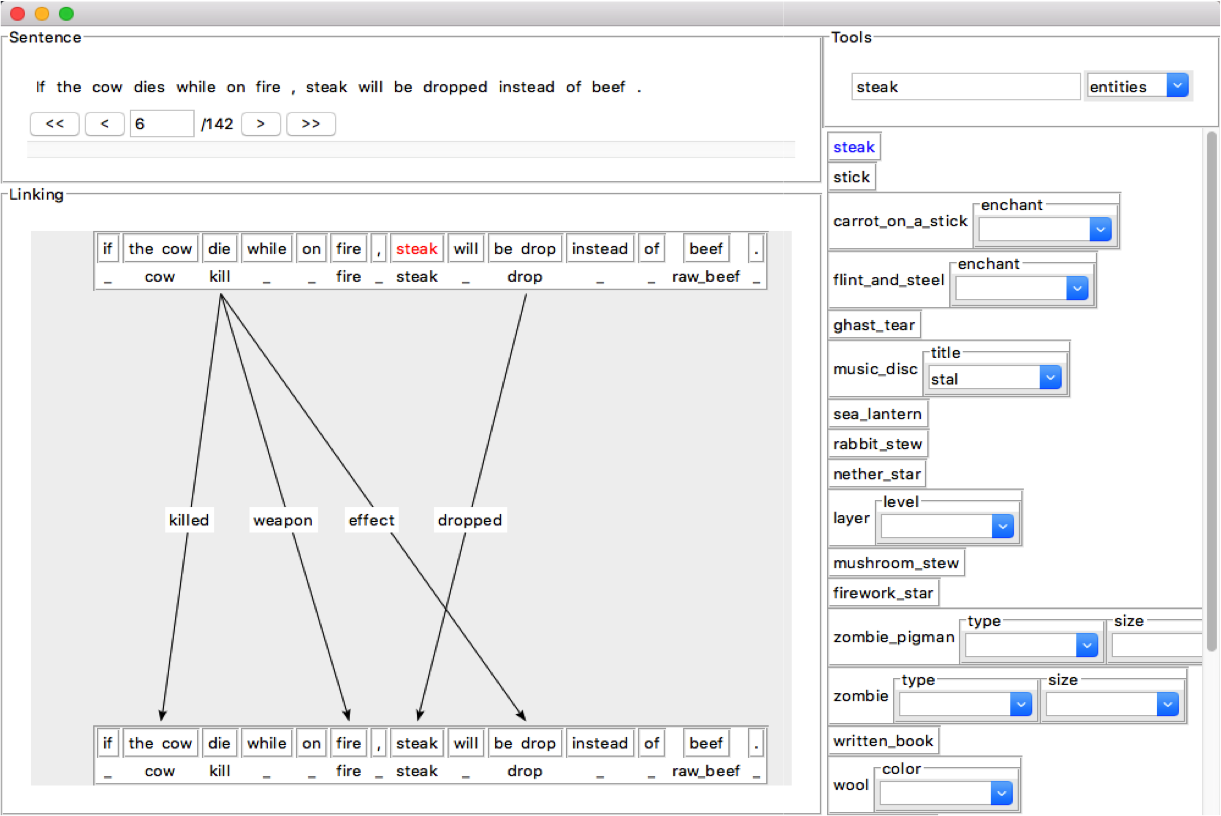
\includegraphics[width=\linewidth]{Figures/Knowledge/annot_tool.png}
   \caption{\label{annot_tool} Annotation tool}
\end{figure}
s it contains the ontology, this tool can propose the possible labels to the annotator, in order to simplify the annotation process and to ensure that the annotation respects the ontology constraints.\\
Using this tool, we manually annotated 301 samples of instances (142 positive examples and 159 negative examples) and 485 samples of relations (266 positive examples and 219 negative examples).\\
Furthermore, we also created 6471 automatic samples of instances (positive examples only) from the anchors contained in the extracted knowledge corpus. Indeed, such as Wikipedia, the 3 websites we extracted knowledge from contain a lot of hyperlinks that lead to an other page of the same website, called anchors. These anchors then link a fragment of text to the title of an other page. If the title of the page pointed by a hyperlink can be identify as the name of an instance class in the ontology, the fragment of text that holds the hyperlink becomes a positive example for this instance class, and can be added to the training dataset.

\subsection{Conclusion on the data collection}

In this section, we first have described a knowledge database and a question answering corpus related to the video game Minecraft. We have shown that even for low resource domains, data can be extracted from the web, by designing adapted extracting rules.\\
We saw that the extracted structured data can be used to make the definition of an ontology easier.\\
And we saw that the textual data can be used to create a training dataset for a semantic parser, and that this training dataset can be completed automatically with instances samples by using websites anchors. We will show in the following section on semantic parsing that we can also use textual data to train embedding models that we will use to improve the performance of the semantic parser.\\

Our final goal is to use the collected data to build a system that can answer questions using the logic specific to the game. A lot of research has been done on the answering of real world questions using Freebase \cite{berant2014semantic,yao2015lean} or Wikipedia \cite{pasupat2015compositional}. Datasets for these tasks usually favour systems that do simple queries of facts on the knowledge database \cite{yao2015lean}. As the complexity of the questions increases, answering the questions usually becomes considerably difficult \cite{pasupat2015compositional}, due to the vast complexity of the real world. Our purpose is to show that in restricted domains with a strict logic, such as video games, even difficult questions can be addressed, and this by using only a very limited quantity of annotated resource. This will be the point of the following sections.

\newpage
\section{Semantic Parsing}

In the context of our study, \textbf{semantic parsing} is a process that take a sentence as input and outputs a knowledge graph that represents the meaning of the sentence (see Figure~\ref{semanticParsingFigure}).

\begin{figure}[!ht]
	\centering 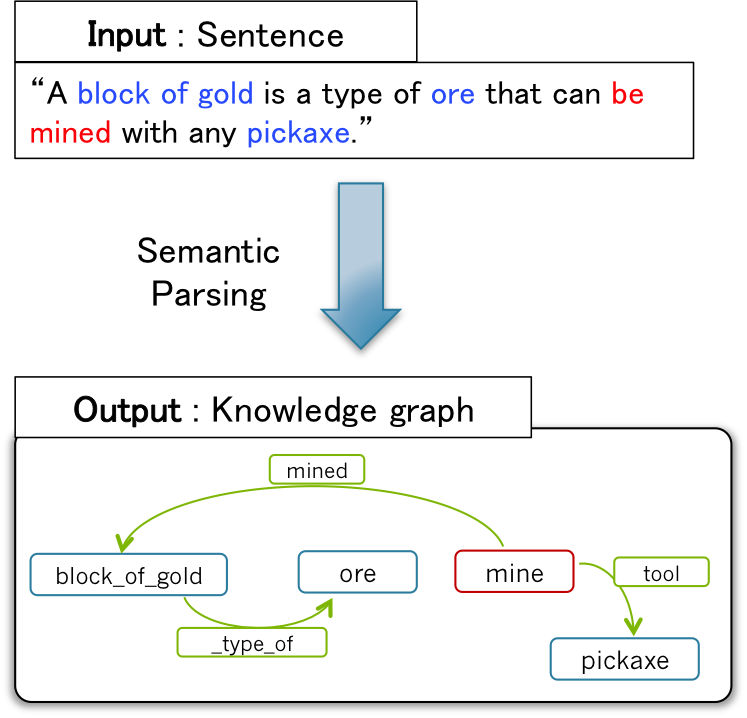
\includegraphics[width=0.55\textwidth]{Figures/Semantic_Parsing/semanticParsingFigure.png}
	\caption{\label{semanticParsingFigure}Semantic Parsing}
\end{figure}

The knowledge graph is composed of instances (the nodes) and relations (the edges) that belong to the ontology that we defined previously.\\
The knowledge graph is constructed in two steps, the instance classification that generates the nodes (in red and blue), and the relation classification that generates the edges (in green).\\
There is an other process called \textbf{syntactic parsing} that, like semantic parsing, generates an output graph (the syntactic tree, see Figure~\ref{syntacticTree}) from an input sentence, but, contrary to semantic parsing, this graph does not represent the meaning of the sentence but its syntax. Nodes are the words of the sentence, and edges are the syntactic dependencies between these words.

\begin{figure}[!ht]
	\centering 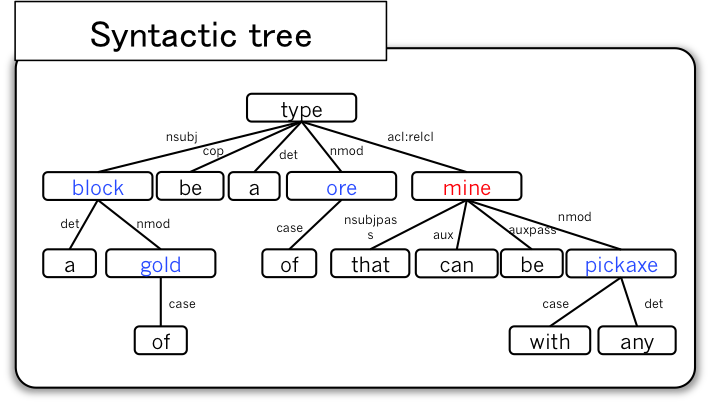
\includegraphics[width=0.65\textwidth]{Figures/Semantic_Parsing/syntacticTree.png}
	\caption{\label{syntacticTree}Syntactic tree of the sentence ``A block a gold is a type of ore that can be mined with any pickaxe''}
\end{figure}

We can notice a similarity between the knowledge graph and the syntactic tree. Thus, our idea was to use the information contained in the syntactic tree as a base for the semantic parsing. In particular, using the words (nodes of the syntactic tree) in the instance classification step, and the syntactic dependencies (edges of the syntactic tree) in relation classification step.\\
The syntactic parsing process does not depend on a domain ontology; it has been largely studied in the past and performing syntactic parsers have been released by NLP researchers \cite{chen2014fast,andor2016globally}. So we can easily apply existing syntactic parsers to our work, and use syntactic trees in our semantic parsing.

\subsection{Instance classification}

Instance classification is the classification of a phrase (a group of words) into an instance class from the ontology. So we need to extract features to classify from phrases. Word embedding has been shown to produce non-sparse and effective features to represent the meaning of words \cite{mikolov2013efficient}.

\subsubsection{Word Embedding}

Therefore, we trained a word embedding model using as a training corpus the knowledge corpus extracted before, which is a corpus of words sequences specific to Minecraft, with the skip-gram model of the Word2Vec library \cite{mikolov2013distributed}. We obtain a model that produce similar vectors for words with a similar meaning in the context of Minecraft.

\begin{figure}[!ht]
   \centering 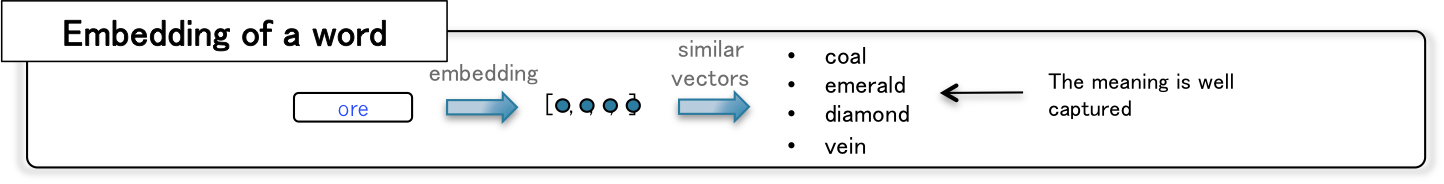
\includegraphics[width=\linewidth]{Figures/Semantic_Parsing/wordEmbedding.png}
   \caption{\label{wordEmbedding} Embedding of the word ``ore''}
\end{figure}

Then, the embedding representation of a phrase using our Word2Vec model is calculated as the average vector of the embedding representation of all words in the phrase.\\
The challenging point is to create, from a word embedding model, a model that embed correctly the meaning of a phrase. Our Word2Vec based phrase embedding model does not include the different importance of the words in natural language (e.g. in ``a baby villager'', the word ``villager'' is more important to catch the meaning of the instance described than the word ``baby''). This difference between the importances of each word in a phrase is visible in the syntactic tree that represents this phrase. The most important word is the root of the tree, which is specified by its children nodes, and deepest nodes have least importance.\\
In other words, it could be interesting to include, in the embedding of a phrase, the syntactic pattern followed by the words, which is a quite difficult task \cite{takase2016modeling}.
However, more specifically, we can keep an information on the syntactic relations between the words by using the VecDCS library \cite{tian2016learning}. In this method, the embedding representation of a phrase is calculated using the DCS tree representation of the phrase that can be obtained from the syntactic tree (Figure~\ref{dcsTree}).

\begin{figure}[!ht]
   \centering 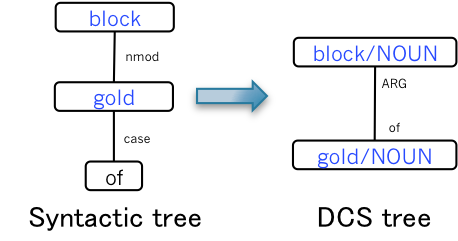
\includegraphics[width=0.3\linewidth]{Figures/Semantic_Parsing/dcsTree.png}
   \caption{\label{dcsTree} DCS tree of the phrase ``block of gold''}
\end{figure}

And the VecDCS embedding of the phrase can be calculated from the individual embedding vectors of the different nodes of the DCS tree by the formula given in Figure~\ref{vecDCSFormula}.
%$v_{node}=v_{node}+\dfrac{1}{n}\sum\limits_{child}^nv_{child}M_{ul_{child}}M_{ol_{child}}^{-1}$

\begin{figure}[!ht]
   \centering 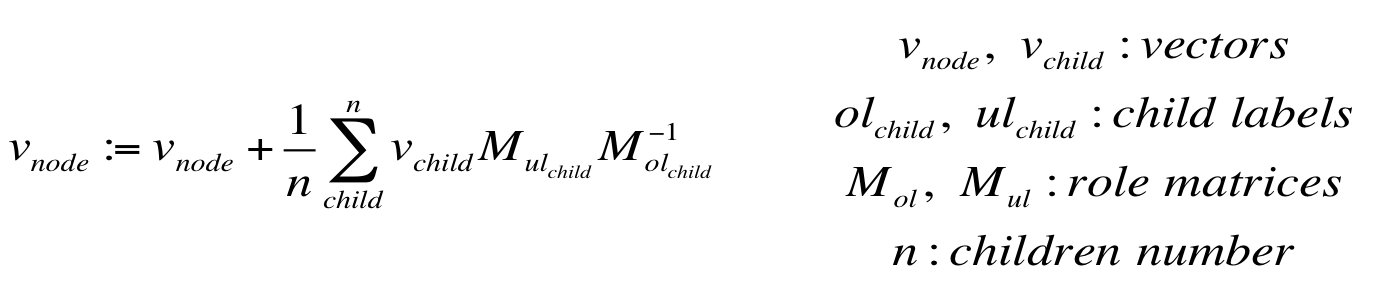
\includegraphics[width=\linewidth]{Figures/Semantic_Parsing/vecDCS.png}
   \caption{\label{vecDCSFormula} Formula of the VecDCS embedding vector of a syntactic sub-tree}
\end{figure}

Therefore, we also trained a VecDCS model for Minecraft, using the extracted knowledge corpus.
We dispose of two different phrase embedding models that can be use to produce features for instance classification (Word2Vec model and VecDCS model).

\begin{figure}[!ht]
   \centering 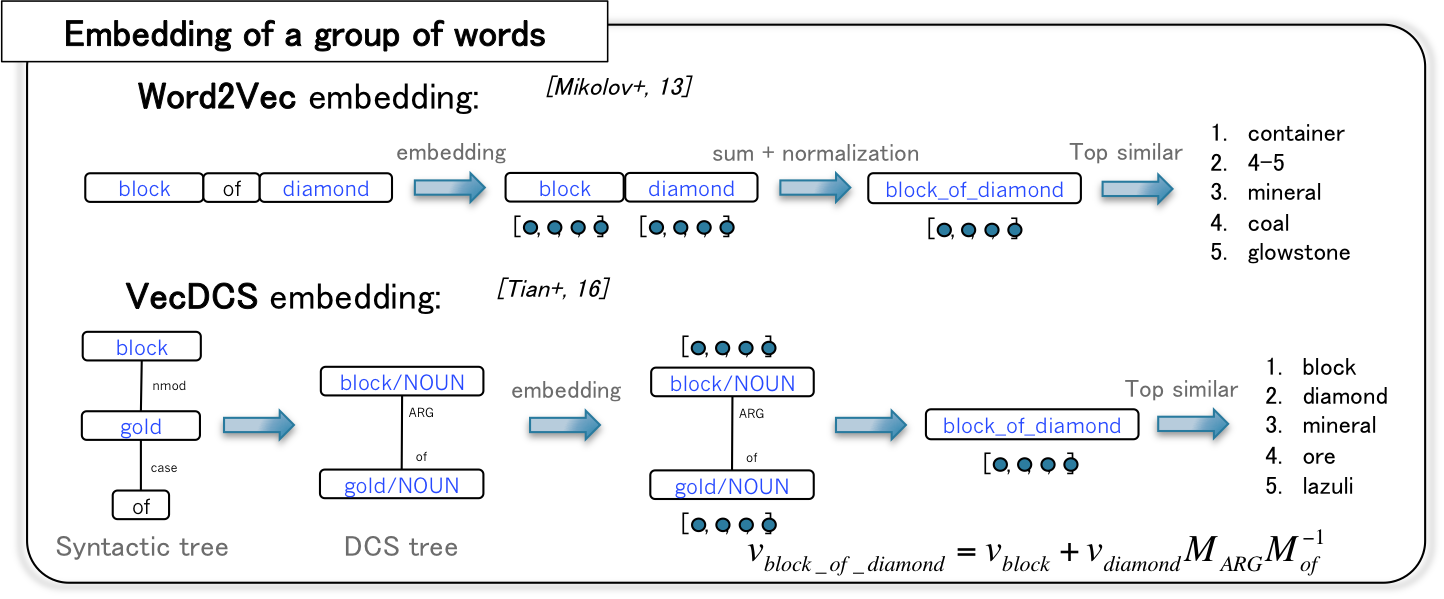
\includegraphics[width=\linewidth]{Figures/Semantic_Parsing/groupWordEmbedding.png}
   \caption{\label{groupWordEmbedding} Two phrase embedding models}
\end{figure}

Our experiment in instance classification will, then, also be a way to study the performance of each embedding model (the VecDCS model being expected to produce more effective features).

\subsubsection{Models for Instance Classification}

We defined two baseline models for the instance classification step.
The first one uses a string similarity method (we refer to it as StringSim). It does not use embedding models to classify words. We just compare the words of the phrase to classify with the names of every instance classes in the ontology, and chose the closest instance class as the prediction for the phrase. To calculate the string similarity between two phrases (the name of an instance class of the ontology is also a phrase/group of words), we use a combination of the Levenshtein distance and the Hungarian algorithm (an alignment algorithm) to align words.\\
In details (see Figure~\ref{distance}), we create a matrix with as many rows as there are words in the first phrase and as many columns as there are words in the second phrase. We add an additional row and an additional column that correspond to the empty word (so that we can align a word on the empty word and have a different number of words in the two groups). Then we fill the cells of the matrix with the Levenshtein distance between words of the two phrases. Finally, we use a variation of the Hungarian algorithm to find the alignment of words that minimize the sum of the distances. The variation allows aligning any number of words (include no word) on the empty word. The result of this Hungarian algorithm on the constructed matrix is the distance between the two phrases (see Figure~\ref{distance}). If all words are aligned on the empty word (the cost of creating a word is smaller than the transformation of a word of the other group to this word), then there is no similarity between the two phrases and the distance in set to infinite.

\begin{figure}[!ht]
   \centering 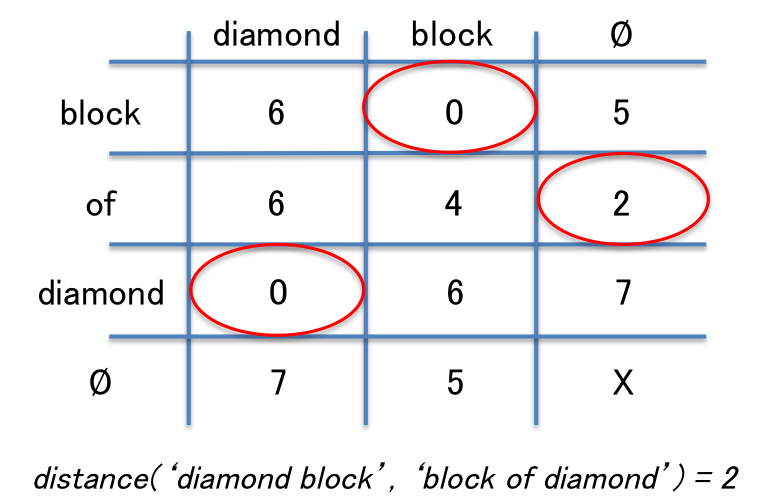
\includegraphics[width=0.65\linewidth]{Figures/Semantic_Parsing/distance.png}
   \caption{\label{distance} Distance between 'diamond block' and 'block of diamond'}
\end{figure}

Note that even if the distance is infinite for distant phrases, we can fix a finite upper limit on the acceptable distance between a phrase to classify and the names of classes. Over this limit, or threshold, even if a class name is the closest to the phrase among all classes, the phrase will not be classified with this class. This threshold is the only parameter of the StringSim model.

The second baseline, Flat SVM model (Figure~\ref{flatSVMModel}), uses the simple Word2Vec embedding model to extract features from a phrase, and we classify the features with a multi-class RBF kernel SVM classifier that outputs one of the 508 instance classes of the ontology, or null if the group of words does not represent an instance.

\begin{figure}[!ht]
   \centering 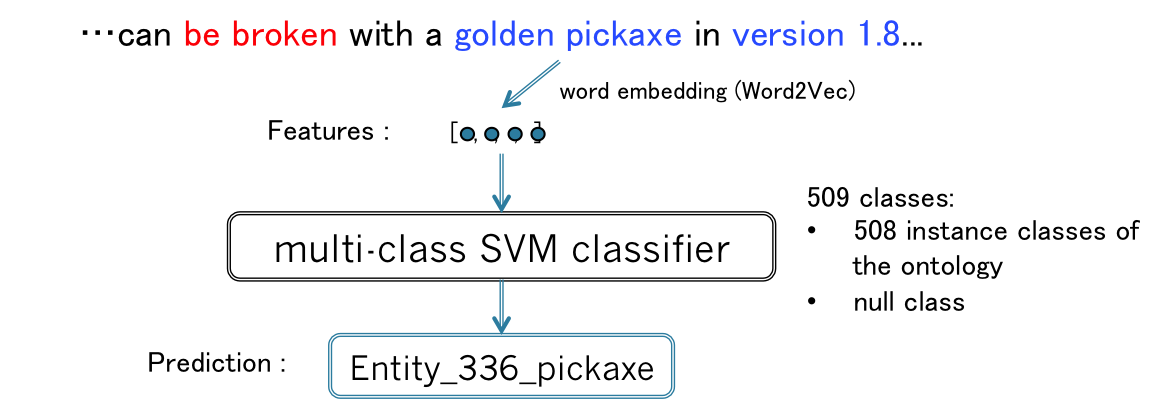
\includegraphics[width=0.7\linewidth]{Figures/Semantic_Parsing/flatSVMModel.png}
   \caption{\label{flatSVMModel} Flat SVM model for instance classification}
\end{figure}

This model uses a C-SVC RBF kernel SVM (support vector machine) classifier implemented in the LIBSVM library \cite{chang2011libsvm} (this is also the library that we used for the other models using SVM classifiers in this work). This classifier is defined by two parameters called $c$ (for cost) and $gamma$ (that defines the kernel function of the classifier). Hence, the training of the Flat SVM model depends on the these two hyper-parameters $c$ and $gamma$.\\
During the training, for each class, we use positive and negative training samples. The positive samples of a class are the positive examples of the training dataset for this class and the negative samples of a class are the negative examples (not an instance) of the training dataset and the positive examples of the other classes.

Then, we defined an improved model called Hierarchical SVM model (Figure~\ref{hierarchicalSVMModel}). This is an improvement of the Flat SVM model in which we integrate the ontology's hierarchy of instances. We still use a phrase embedding model to extract features from phrases. But we do not classify the features with one multi-class SVM classifier. We classify features recursively, following the ontology's hierarchy, using one binary RBF kernel SVM classifier for each instance class. To classify a phrase, we check at first if it belongs or not to the ENTITY class and to the EVENT class, which are the two roots of the instances hierarchy, using their respective binary classifiers. If and only if it is predicted as belonging to a class, we check the belonging to the children classes (object, version, \emph{etc.}) and continue recursively. If the phrase doesn't belong to any children class, the recursion ends and the phrase is classified as the last predicted class. Note that we can obtain several predictions using this process. However, we can rank the several predictions by outputting the probabilities for each binary classifier's prediction. The probability of a prediction is defined as the geometric mean of the probabilities output by each binary classifier in the recursion. For example, in Figure~\ref{hierarchicalSVMModel}, the probability of the prediction as \textit{pickaxe} is:
\begin{quote}
$P(Entity\_336\_pickaxe) =$\\
$	(P(ENTITY)*P(object)*P(item)*P(tool)*P(pickaxe))^{1/5}$
\end{quote}

\begin{figure}[!ht]
   \centering 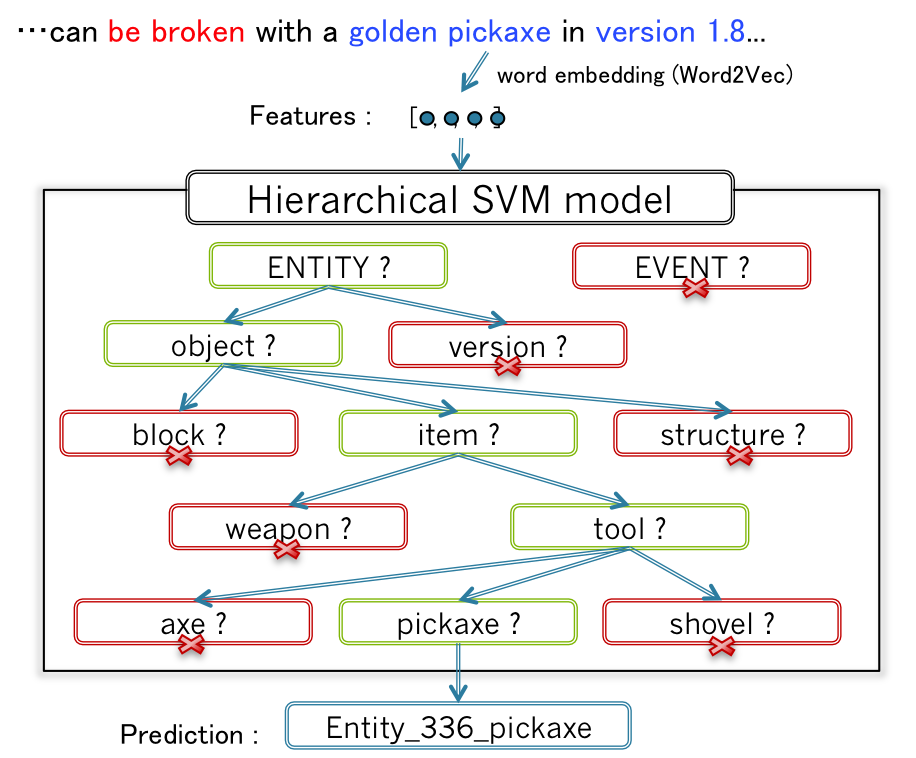
\includegraphics[width=0.7\linewidth]{Figures/Semantic_Parsing/hierarchicalSVMModel.png}
   \caption{\label{hierarchicalSVMModel} Improvement: Hierarchical SVM model for instance classification}
\end{figure}

As for the Flat SVM model, this model uses C-SVC RBF kernel SVM classifiers, so the training depends on two hyper-parameters $c$ and $gamma$. Furthermore, as we output the probabilities of binary classifiers' predictions, we can define a threshold on the probability to decide if yes or no a phrase belong to a class. We can define a local threshold (we will refer to it as $threshold$) that must be respected by the binary classifiers' predictions at each step of the recursive prediction, and a global threshold that must be respected by the geometric mean of all probabilities on the whole prediction (we call it cumulative threshold, and will refer to it as $cumul$ for short). Then the training of the Hierarchical SVM model depends on 4 hyper-parameters: $c$, $gamma$, $threshold$ and $cumul$.\\
During the training, for each class, we use positive and negative training samples. The positive samples of a class are the positive examples of the training dataset for this class and for all the descendent classes in the ontology's hierarchy. The negative samples of a class are only the positive examples of the sibling classes and the direct parent classes, except for the roots of the hierarchy (ENITITY\_0 and EVENT\_0) for which the negative samples are the negative examples (not an instance) of the training dataset.

\subsubsection{Tuning of Hyper-parameters}

We tuned the hyper-parameters for each model by comparing their performance in terms of F1-score (micro and macro values) on the training dataset for different values of the hyper-parameters and by choosing the values that lead to the best performance. While the StringSim model's performance is measured using the whole dataset for testing, the other models have to be trained, so we measured their performance through a 2-1 cross-validation (2/3 training and 1/3 testing).

\begin{figure}[!ht]
   \centering 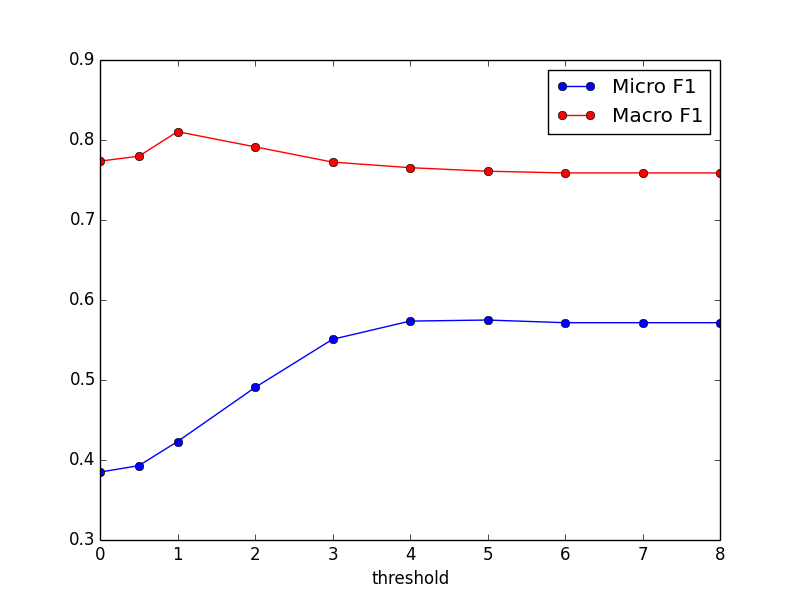
\includegraphics[width=0.7\linewidth]{Figures/Tuning_Figures/instanceClassification_stringSim_tuning.png}
   \caption{\label{stringSimTuning} Distance threshold tuning for the StringSim model}
\end{figure}

The results of the tuning for the StringSim model (Figure~\ref{stringSimTuning}) shows that the distance threshold, when set to a small value (strict similarity), can be useful to increase the precision of the classification (ensure that the predictions are correct). However, small values of the threshold decrease the recall of the classification, because it penalizes the frequent classes that have a high lexical diversity. The values of $threshold=1$ (strict similarity) and $threshold=4$ (soft similarity) for the threshold have been kept for this baseline to do a comparison between the several instance classification models.

For the Flat SVM model, we tuned $c$ and $gamma$ together by comparing the performance of the model for different couples $(c, gamma)$ (Figure~\ref{flatKernelTuning}).

\begin{figure}[!ht]
    \centering
    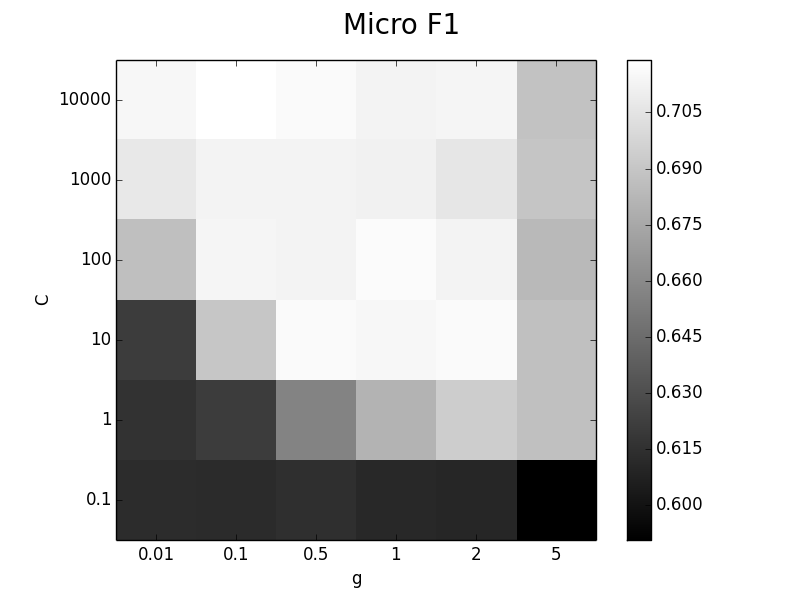
\includegraphics[width=0.5\linewidth]{Figures/Tuning_Figures/instanceClassification_flat_tuning_Micro_F1.png}\hfill
    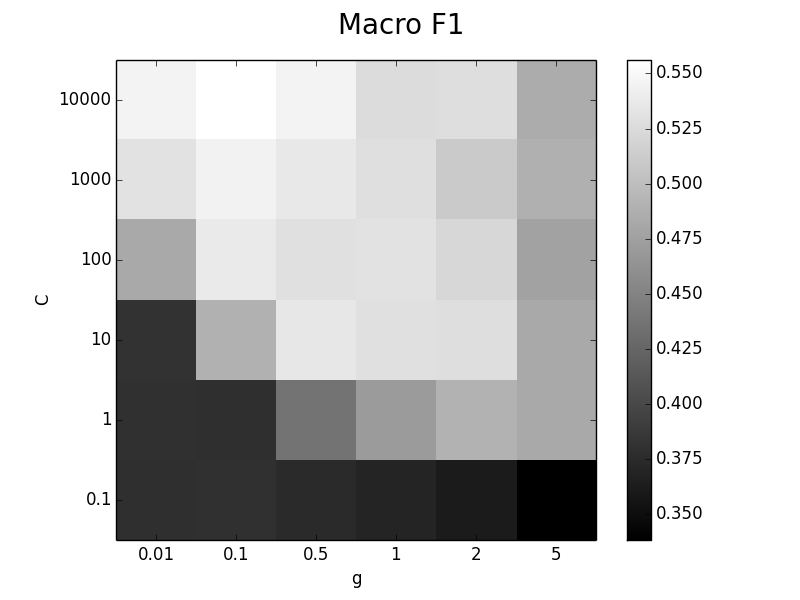
\includegraphics[width=0.5\linewidth]{Figures/Tuning_Figures/instanceClassification_flat_tuning_Macro_F1.png}
    \caption{\label{flatKernelTuning} Hyper-parameters tuning for the Flat SVM model}
\end{figure}

We kept the values $(c=10000, gamma=0.1)$ to optimize the performance.

For the Hierarchical SVM model, we made the assumption that we can tune $c$, $gamma$ independently from $threshold$ and $cumul$ because they do not affect the same part of the model\footnote{The validity of this assumption is not evaluated in this study and should be part of future works.} and it is far easier to tune couples of hyper-parameters than tuples of 4 hyper-parameters. Then we tuned $c$ and $gamma$ first for default values of $(threshold=0.5, cumul=0.5)$, and tuned $threshold$ and $cumul$ afterwards with the best values for $c$ and $gamma$ (Figure~\ref{hierarchicalKernelTuning}).

\begin{figure}[!ht]
    \centering
    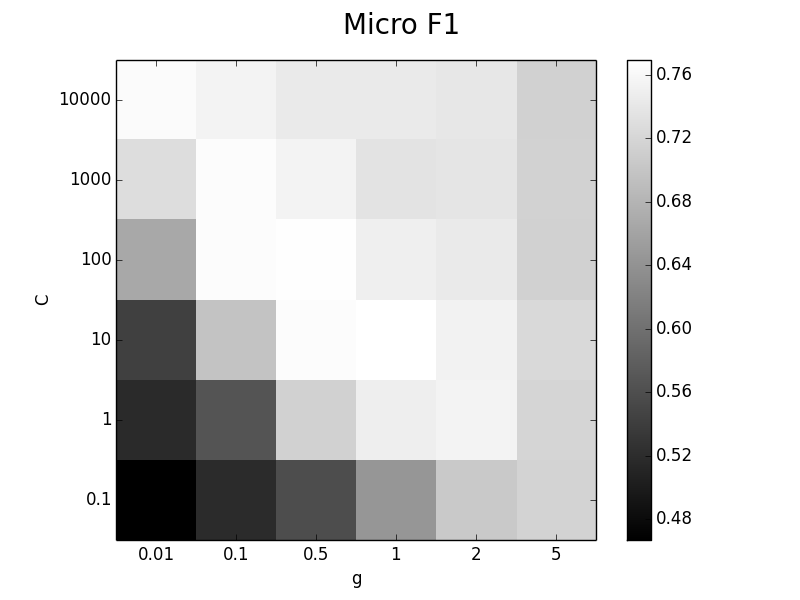
\includegraphics[width=0.5\linewidth]{Figures/Tuning_Figures/instanceClassification_kernel_tuning_Micro_F1.png}\hfill
    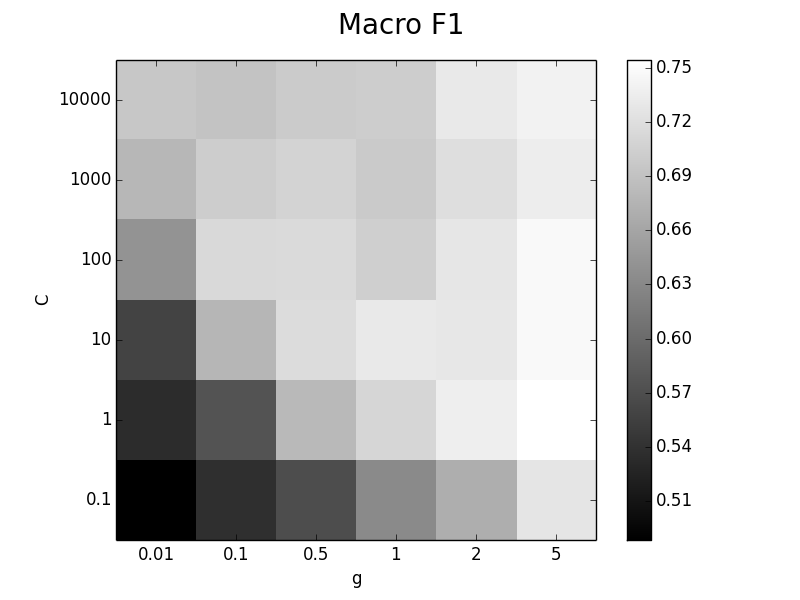
\includegraphics[width=0.5\linewidth]{Figures/Tuning_Figures/instanceClassification_kernel_tuning_Macro_F1.png}\vfill
    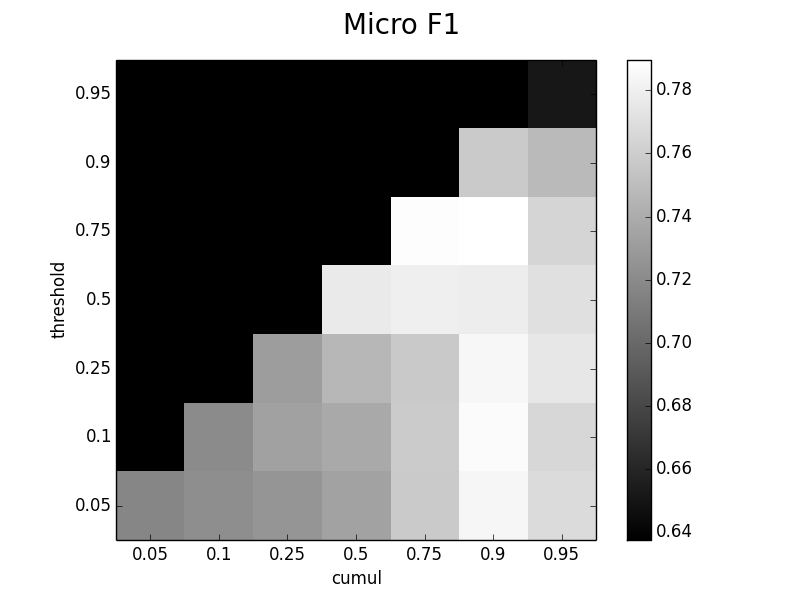
\includegraphics[width=0.5\linewidth]{Figures/Tuning_Figures/instanceClassification_threshold_tuning_Micro_F1.png}\hfill
    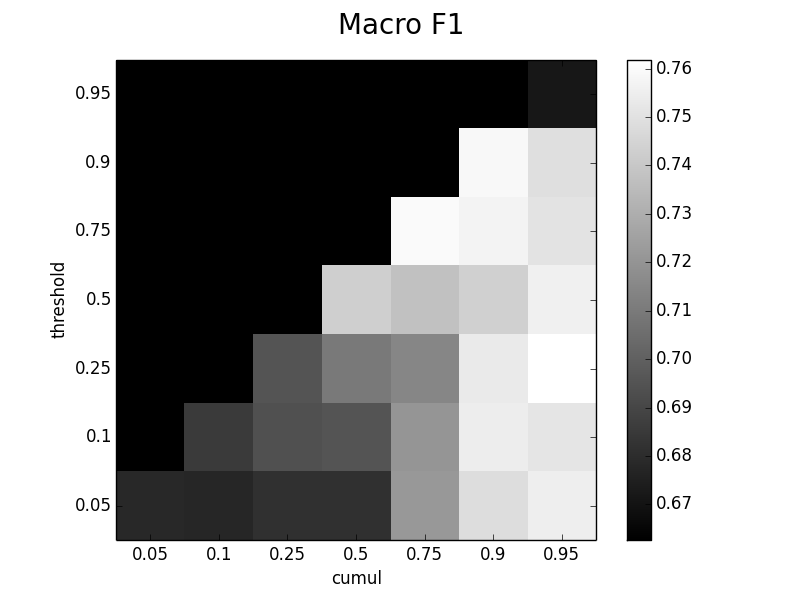
\includegraphics[width=0.5\linewidth]{Figures/Tuning_Figures/instanceClassification_threshold_tuning_Macro_F1.png}
    \caption{\label{hierarchicalKernelTuning} Hyper-parameters tuning for the Hierarchical SVM model}
\end{figure}

From the results of the tuning for the Hierachical SVM model, we first chose $(c=10, gamma=1)$ to optimize the micro F1-score (the performance on frequent classes of the ontology). We can notice that these values are not optimal in term of macro F1-score (performance giving importance to rare classes), but the loss on macro F1-score when optimizing micro F1-score is lower than the loss on the micro F1-score in the case where we optimize the macro F1-score. Furthermore, the value that is usually used for $gamma$ is the inverse of the number of features used in the classification. As we use only one feature, which is the normalized embedding vector of a phrase, this value of $gamma=1$ was expected to be optimal a priori.
Then we tune the $threshold$ and the $cumul$ for $(c=10, gamma=1)$. The couple $(threshold=0.75, cumul=0.9)$ gives the best performance for micro-F1-score and one of the best macro F1-score. Note that the tuning is not done in the region $threshold > cumul$, because in this case, by definition of the cumulative threshold, any prediction that respects the local threshold at each step must necessarily respects the cumulative threshold, so $cumul$ is not a relevant hyper-parameter anymore. The diagonal $threshold = cumul$ then gives the result of the tuning for the $threshold$ hyper-parameter alone. On the contrary, when $threshold < cumul$, a phrase can be classified as an instance class even if the prediction from a binary classifier was low at some step of the recursion as long as the whole probability is high. Finally, we kept the values $(c=10, gamma=1, threshold=0.75, cumul=0.9)$. These values will be used for the Hierarchical SVM model independently of the phrase embedding model used to produce the features to classify, which is an other strong assumption that would need to be verified in future works.\\

\subsubsection{Experimental results for Instance Classification}

We used the training dataset built before to train models (except StringSim that does not require training), and to test them through a 2-1 cross-validation.
We calculated the micro F1-score and the macro F1-score for each model. Results are presented in Table~\ref{resultsInstanceClassification}. The micro F1-score can be considered as the performance of the model on frequent classes and the macro F1-score gives the same importance to frequent and rare classes, so the difference between micro and macro F1-scores gives an idea of the difference of performance between frequent and rare classes.

\begin{table}[!ht]
\center
\begin{tabular}{c||c|c}
	Model & Micro F1 & Macro F1 \\
	\hline
	\hline
	strict StringSim & 0.423 & 0.810 \\
	(threshold = 1) & & \\ \hline
	soft StringSim & 0.574 & 0.765 \\
	(threshold = 4) & & \\ \hline
	Flat SVM Model & 0.719 & 0.556 \\
	(Word2Vec embedding) & & \\ \hline
	Hierarchical SVM Model & 0.791 & 0.761\\
	(Word2Vec embedding) & & \\ \hline
	Hierarchical SVM Model & \textbf{0.869} & \textbf{0.855}\\
	(VecDCS embedding + context features) & & \\
\end{tabular}
\caption{\label{resultsInstanceClassification} Experimental results for Instance Classification}
\end{table}

\begin{table}[!ht]
\center
\begin{tabular}{c||c|c}
	Model & Macro Precision & Macro Recall \\
	\hline
	\hline
	strict StringSim & 0.929 & 0.719 \\
	(threshold = 1) & & \\ \hline
	soft StringSim & 0.715 & \textbf{0.823} \\
	(threshold = 4) & & \\ \hline
	Flat SVM Model & \textbf{0.955} & 0.392 \\
	(Word2Vec embedding) & & \\ \hline
	Hierarchical SVM Model & 0.801 & 0.724\\
	(Word2Vec embedding) & & \\ \hline
	Hierarchical SVM Model & 0.896 & 0.817\\
	(VecDCS embedding + context features) & & \\
\end{tabular}
\caption{\label{recallInstanceClassification} Precision and recall for Instance Classification}
\end{table}

By comparing the two baselines (StringSim and Flat SVM model), we can see that the Flat SVM model, that uses embedding features is more performing on frequent classes, because frequent classes have more lexical diversity, and then classifying the meaning of words is better than classifying the surface of words. However, the Flat model uses only one SVM classifier for more than 500 classes, and as a result, rare classes are not correctly learnt even if this model has the best macro precision. This can be seen through its very low recall in Table~\ref{recallInstanceClassification}, or by looking at the confusion matrix of the classification in Figure~\ref{flatConfusion}.\\

\begin{figure}[!ht]
   \centering 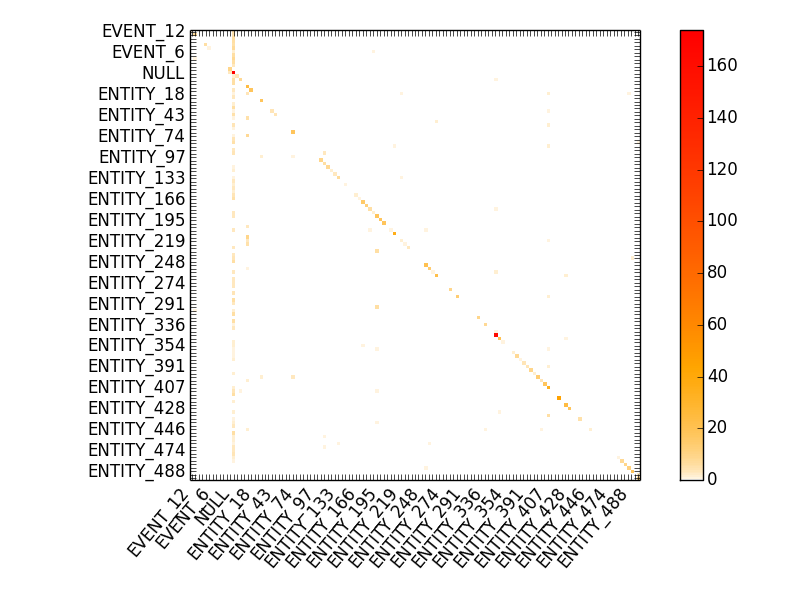
\includegraphics[width=0.8\linewidth]{Figures/Confusion_Matrices/confusionMatrixInstanceClassificationGlobal_flat.png}
   \caption{\label{flatConfusion} Confusion matrix of instance classification with the Flat SVM model}
\end{figure}

But if we compare the Flat SVM model with the Hierachical SVM model when using the Word2Vec phrase embedding model, we can see that we make a large improvement on rare classes by using the hierarchy of instances, as the gap between micro and macro F1-score largely decreases. Still, it is not sufficient to beat the String Similarity baseline in term of macro F1-score.\\
However, we could improve the performance of the Hierachical SVM model by changing the embedding model used to extract features from the phrase to classify. Instead of using the phrase embedding model based on Word2Vec word embedding alone, we use a combination of it with the more elaborate phrase embedding model based on VecDCS word embedding. The phrase embedding model based on VecDCS is used to extract a feature vector from the phrase to classify, and the phrase embedding model based on Word2Vec is used to extract a feature vector from the context of the phrase. To do so, we apply the Word2Vec phrase embedding model on the bag of words constituted with the words located at the nodes of the syntactic tree that are directly adjacent to at least one node that is part of the phrase to classify. The concatenation of these two vectors of features is used to classify the phrase. In this case, we use $gamma=0.5$ as hyper-parameter, as we use two different set of features. With this model, we obtain the best performance for both micro and macro F1-scores. And if we look at the Table~\ref{recallInstanceClassification}, we can see that the good performance of the Hierarchical SVM model is due to a good balance between precision and recall.

\subsubsection{Conclusion on Instance classification}

As a conclusion on instance classification, we have shown that:
\begin{itemize}
\item Word embedding models are useful in the classification of frequent instance classes with high lexical diversity.
\item Using the ontology's hierarchy is useful to learn to classify correctly rare instance classes.
\item We can use elaborate features (VecDCS embedding features and context features) to obtain the best performance on the instance classification task.
\end{itemize}

\subsection{Relation classification}

Relation classification is the classification of the syntactic paths of a syntactic tree into relation classes from the ontology. 
Similarly to what we saw in the section on word embedding, convert syntactic paths to their vector representation could be an efficient way to produce features to classify with a SVM model.

\subsubsection{Dependency Embedding}

We need an embedding model for syntactic paths that will produce similar vector representations for similar paths. The question is then, what are similar paths?\\
As syntactic paths are sequences of words and syntactic dependencies, similar paths will be similar sequences, so it is logical to begin by embedding the elements that compose the sequences: words and syntactic dependencies. We already have a word embedding model, so we need to train a dependencyembedding model that will produce similar vectors for similar dependencies. 
Contrary to words, for which we can find synonyms, each dependency has a distinct syntactic role. However, some dependencies can be closer than others, such as $advcl:when$ (when condition) and $advcl:if$ (if condition), which are closer than $advcl:when$ and $advcl:to$ (consequence, or reversed condition). We can also notice the similarity between single dependencies and bigrams of dependencies (e.g. $nsubj$ and $nsubj\_xcomp^{-1}$), so it can be useful to be able to embed both unigrams and bigrams of dependencies.\\
To embed a dependency, or a bigram of dependencies, we used the skip-gram model implemented in the Word2Vec library (syntactic paths being composed from both words and dependencies, making our dependency embedding vectors similar to word embedding vectors simplify the implementation of the syntactic path embedding model). Training such a model only needs a corpus of dependencies sequences (in other words, syntactic paths), so we parsed a part of the knowledge corpus we extracted before with a syntactic parser, and constituted a corpus of syntactic paths. We produced two syntactic dependency embedding models, the first one embedding dependency unigrams, the other one embedding dependency bigrams. For the second one, when constructing the training corpus of syntactic paths, we divided dependency sequences by bigrams, in order to train the embedding model on bigrams of dependencies.

\begin{figure}[!ht]
   \centering 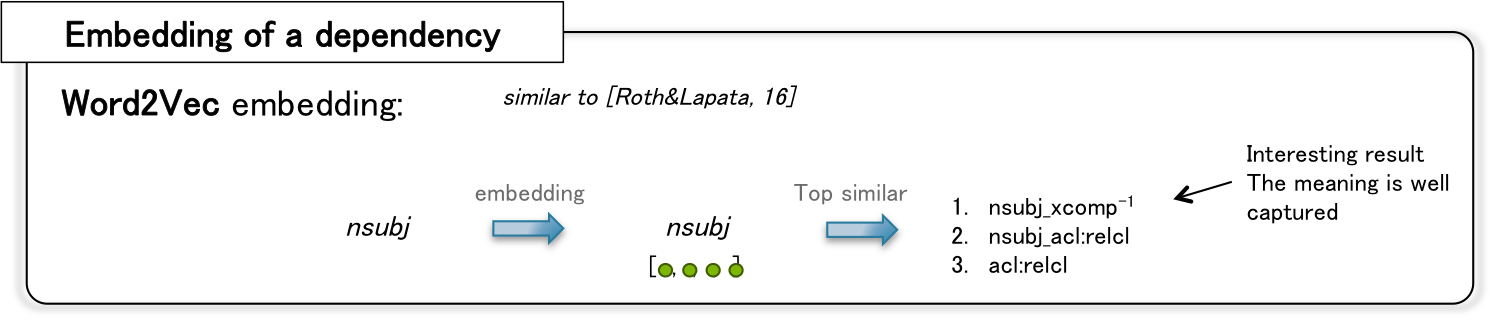
\includegraphics[width=\linewidth]{Figures/Semantic_Parsing/dependencyEmbedding.png}
   \caption{\label{dependencyEmbedding} Embedding of a syntactic dependency unigram}
\end{figure}

To construct a syntactic paths embedding model from a word embedding model and a syntactic dependency embedding model, we begin by dividing the path into two sequences, the sequence of words and the sequence of dependencies.\\
We calculate the embedding vector of the sequence of words by simply calculating the average vector of the embedding representations of all the words in the sequence (the order of the sequence is not used). For the sequence of dependencies, we calculate the average vector of the embedding representations of all dependency unigrams in the path using the first embedding model (the order of the sequence is not used), or of all dependency bigrams in the path using the second embedding model (the order of the sequence is important here).\\
Then we concatenate the embedding representation of the sequence of dependencies and the embedding representation of the sequence of words to obtain the embedding representation of the path.

\begin{figure}[!ht]
   \centering 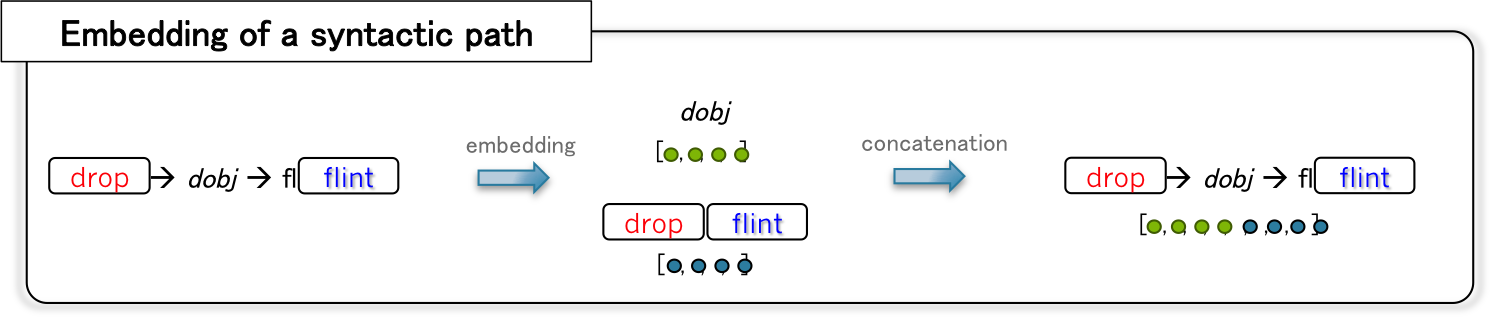
\includegraphics[width=\linewidth]{Figures/Semantic_Parsing/pathEmbedding.png}
   \caption{\label{pathEmbedding} Embedding of a syntactic path}
\end{figure}

We finally dispose of two syntactic path embedding models, one that uses dependency unigram embedding and does not encode the order of the sequence, and an other that uses dependency bigram embedding and then integrates the order of the sequence of dependencies in the syntactic path. If our purpose is similar to the syntactic path embedding done in the work of M. Roth and M. Lapata in 2016 \cite{roth2016neural}, the technology used to construct the model in different. It would then be interesting to compare both approaches in a future work.\\
In our syntactic path embedding models, we also added the possibility not to consider the words in the syntactic path, in which case the path embedding models only embed the sequence of dependencies (unigrams or bigrams).

\subsubsection{Models for Relation Classification}

First, we created a baseline that uses one binary SVM classifier for each relation of the ontology, including the root RELATION of all relations (see Figure~\ref{relationClassificationBaseline}).
After extracting the features from the syntactic path we want to classify with our path embedding model, we begin by testing if the path represent or not a relation of our ontology by classifying it with the root RELATION binary classifier. If the root relation's classifier prediction is positive, we test for each relation class in the ontology if the path belongs to the class or not by using the respective binary SVM classifiers (the classification is then similar to the Hierarchical SVM model for instances in the case of events that have no other hierarchy that the common root). In the example of Figure~\ref{relationClassificationBaseline}), only the \textit{ingredient} relation class is predicted positively.

\begin{figure}[!ht]
   \centering 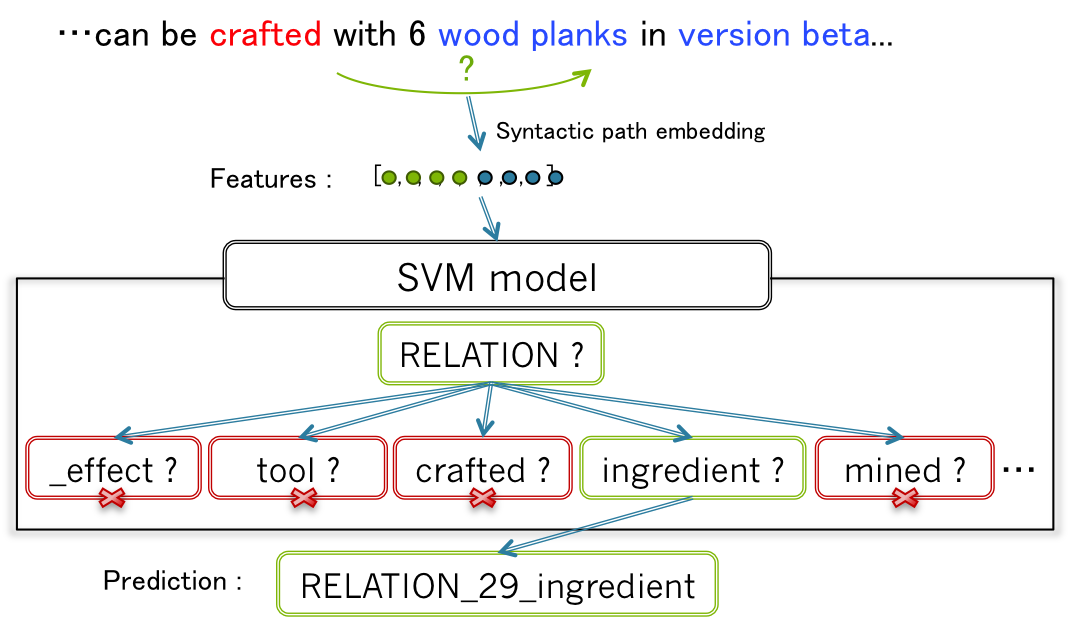
\includegraphics[width=0.7\linewidth]{Figures/Semantic_Parsing/relationClassificationBaseline.png}
   \caption{\label{relationClassificationBaseline} SVM model for relation classification}
\end{figure}

During the training, for each class, we use positive and negative training samples. In the case of the root relation binary classifier, we use all positive examples of the training dataset as positive samples, and all negative examples of the training dataset as negative samples. However, for any other class, the positive samples are the positive examples of the training dataset for this class and the negative samples are the positive examples of the other classes. Using a classifier for the root relation as a first step of the classification instead of testing directly all the relation classes is a way the reduce the number of predictions done by SVM classifiers, and it allows to train relation classes with less negative samples, as the non-relation paths are eliminated by the root classifier at the first step.

We built an improvement of the previous model, by integrating the ontology's constraints into the model (see Figure~\ref{relationClassificationImprovement}).
Indeed, constraints provide useful information when classifying a relation, so we added a constraints verification step at the top of the model.
In other words, before classifying the features of a syntactic path between two entities, we check what relation classes are possible candidates for the relations between these two instances. In the example of Figure~\ref{relationClassificationImprovement}, a relation between ``crafted'' and ``wood planks'' cannot be \textit{\_effect} or \textit{type\_of}, but only \textit{crafted} or \textit{ingredient}. So it is theoretically useless to check if the syntactic path belong to other classes than \textit{crafted} and \textit{ingredient}.

\begin{figure}[!ht]
   \centering 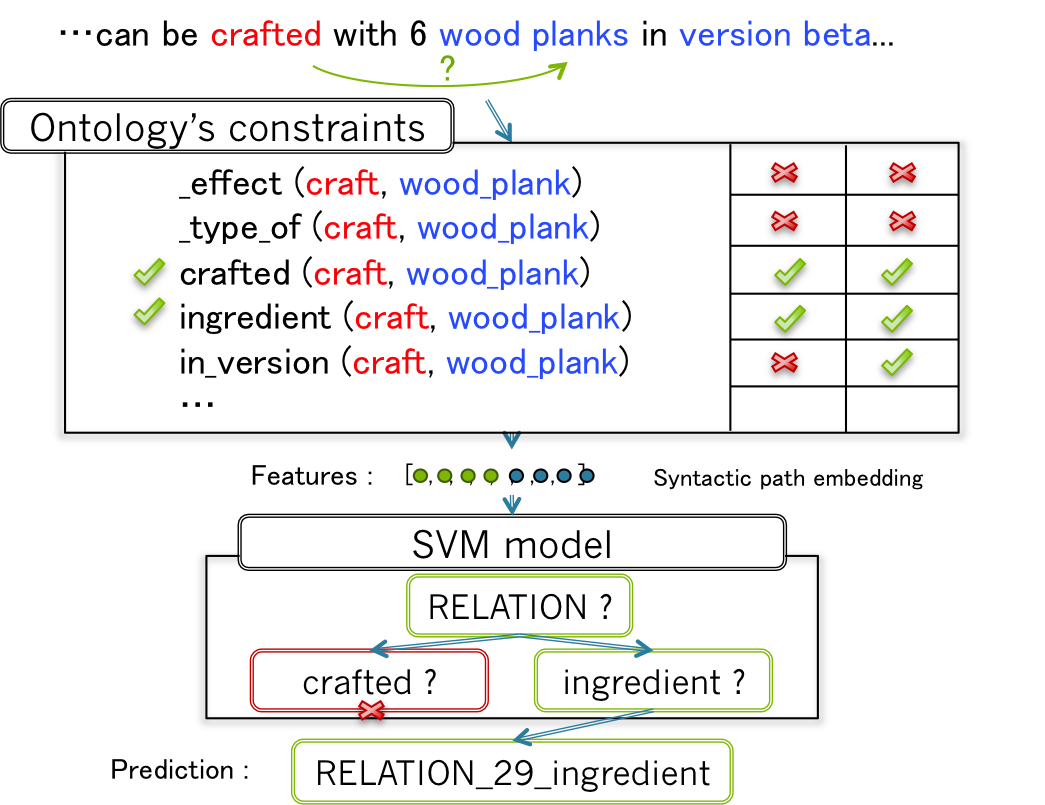
\includegraphics[width=0.7\linewidth]{Figures/Semantic_Parsing/relationClassificationImprovement.png}
   \caption{\label{relationClassificationImprovement} Improvement: SVM model with constraints for relation classification}
\end{figure}

As for the baseline, during the training, for any class except the root, the positive samples are the positive examples of the training dataset for this class, however the negative samples are only the positive examples of the other classes for which this class was also a candidate. The constraints verification step then allows to reduce the number of negative samples even more, which speeds up the training.\\
For each of the two models, we can use either the unigram-based syntactic path embedding model or the bigram-based syntactic path embedding model to produce the features to classify, and for each embedding model, we can consider or not the words of the syntactic paths. In the following section, we will compare both models, but also the difference in performance for each model depending on the syntactic path embedding model that is used to extract features.\\
Such as the Hierarchical SVM model for instance classification, both relation classification models use C-SVC RBF kernel SVM classifiers, so the training depends on two hyper-parameters $c$ and $gamma$. Furthermore, we output the probabilities of binary classifiers' predictions, so we can define a threshold on the probability to decide if yes or no a syntactic path belongs to a relation class. And as the prediction is done in two steps (root classifier and relation classifier), we defined a local threshold ($threshold$) that must be respected by any binary classifier, and a global threshold that must be respected by the geometric mean of the probabilities at the two steps of the prediction (we call it cumulative threshold, $cumul$). Then the training of both models depends on 4 hyper-parameters: $c$, $gamma$, $threshold$ and $cumul$.

\subsubsection{Tuning of Hyper-parameters}

As for the instance classification Hierarchy SVM model, we made the assumption that we can tune $c$, $gamma$ independently from $threshold$ and $cumul$. We also made the assumption that the tuning can be done only ones for both models as the difference is in the constraints verification step and not in the SVM classifiers. Then we tuned $c$ and $gamma$ first for default values of $(threshold=0.2, cumul=0.2)$, and tuned $threshold$ and $cumul$ afterwards with the best values found for $c$ and $gamma$.

\begin{figure}[!ht]
    \centering
    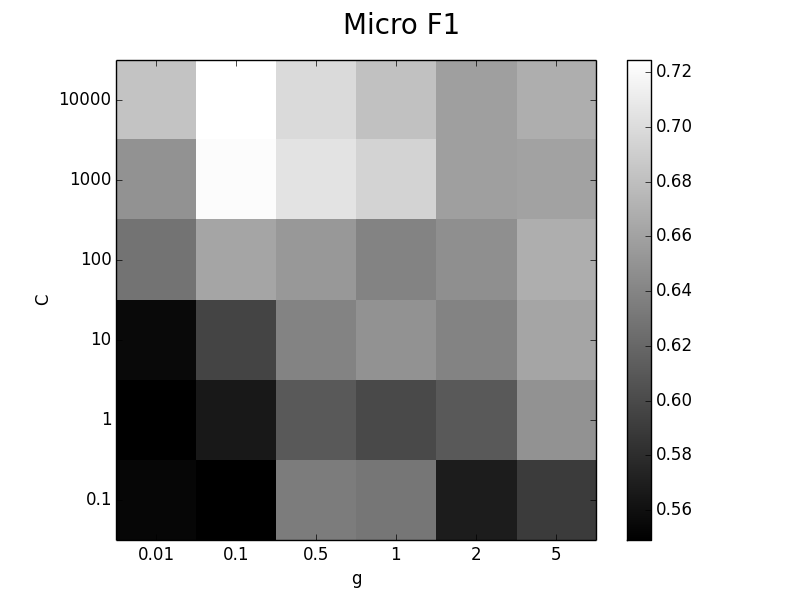
\includegraphics[width=0.5\linewidth]{Figures/Tuning_Figures/relationClassification_kernel_tuning_Micro_F1.png}\hfill
    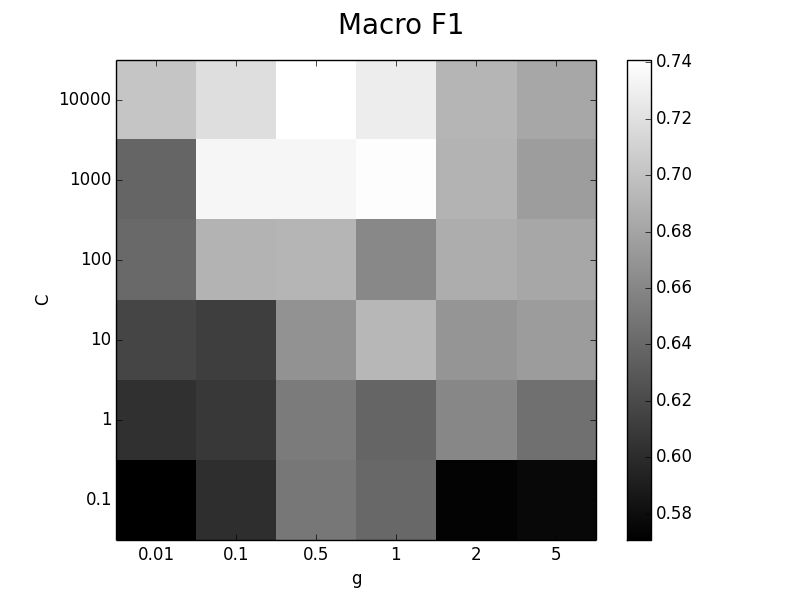
\includegraphics[width=0.5\linewidth]{Figures/Tuning_Figures/relationClassification_kernel_tuning_Macro_F1.png}\vfill
    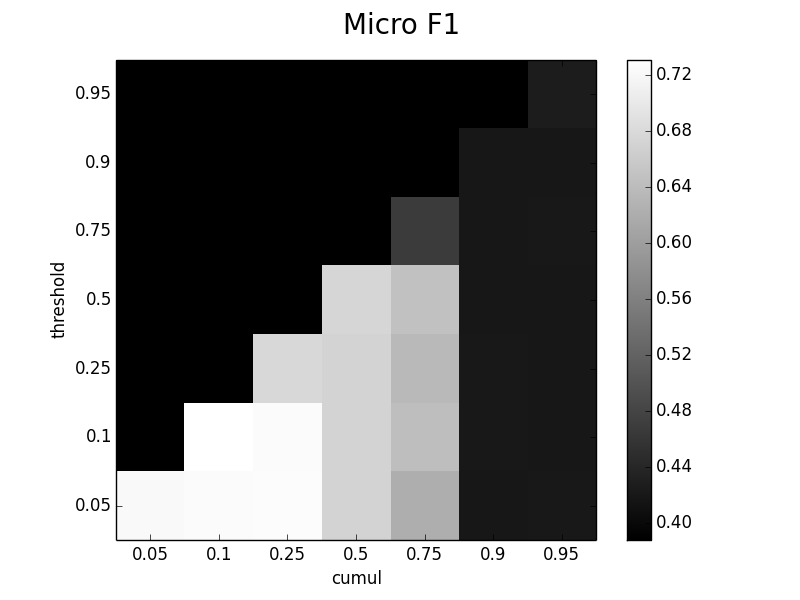
\includegraphics[width=0.5\linewidth]{Figures/Tuning_Figures/relationClassification_threshold_tuning_Micro_F1.png}\hfill
    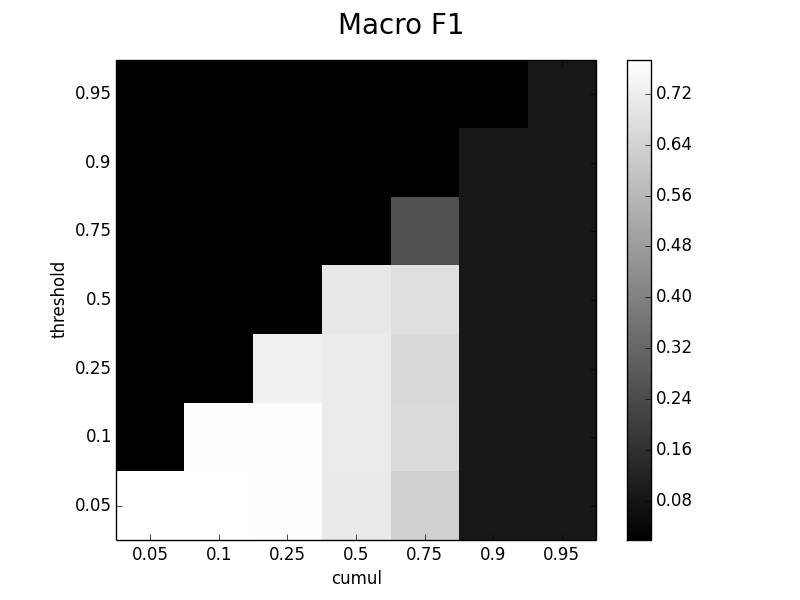
\includegraphics[width=0.5\linewidth]{Figures/Tuning_Figures/relationClassification_threshold_tuning_Macro_F1.png}
    \caption{\label{relationKernelTuning} Hyper-parameters tuning for the Relation Classification models}
\end{figure}

From the results of the tuning, we first chose $(c=10000, gamma=0.5)$ to optimize both micro and macro F1-score.
Then we tune the $threshold$ and the $cumul$ for $(c=10000, gamma=0.5)$. For both micro and macro F1-scores, the couple $(threshold=0.1, cumul=0.1)$ gives the best performance. Note that $threshold=cumul$ means that $cumul$ is a useless hyper-parameter as it will always be respected. Indeed, the geometric mean of two probabilities that must be higher than $threshold$ will also be higher than $threshold$, and then higher than $cumul$. This is also the reason why the tuning is not done in the region $threshold > cumul$. Finally, we kept the values $(c=10, gamma=1, threshold=0.1, cumul=0.1)$.\\

\subsubsection{Experimental results for Relation Classification}

We used the training dataset built before to train and to test our relation classification models (through 2-1 cross-validation). The result of this experiment in presented in Table\ref{resultsRelationClassification}.

\begin{table}[!ht]
\center
\begin{tabular}{c||c|c}
	Model & Micro F1 & Macro F1 \\
	\hline
	\hline
	SVM Model & 0.496 & 0.447 \\
	no constraints, dependency unigrams & & \\ \hline
	SVM Model & 0.501 & 0.456 \\
	no constraints, dependency bigrams & & \\ \hline
	SVM Model & 0.767 & 0.789 \\
	with constraints, dependency unigrams & & \\ \hline
	SVM Model & \textbf{0.792} & \textbf{0.791} \\
	with constraints, dependency bigrams & & \\ \hline
	SVM Model & 0.702 & 0.638 \\
	with constraints, words and dependency bigrams & & \\ \hline
\end{tabular}
\caption{\label{resultsRelationClassification} Experimental results for Relation Classification}
\end{table}

\begin{table}[!ht]
\center
\begin{tabular}{c||c|c}
	 & Macro & Macro \\
	Model & Precision & Recall \\
	\hline
	\hline
	SVM Model & 0.444 & 0.450 \\
	no constraints, dependency unigrams & & \\ \hline
	SVM Model & 0.474 & 0.440 \\
	no constraints, dependency bigrams & & \\ \hline
	SVM Model & \textbf{0.884} & 0.713 \\
	with constraints, dependency unigrams & & \\ \hline
	SVM Model & 0.871 & \textbf{0.725} \\
	with constraints, dependency bigrams & & \\ \hline
	SVM Model & 0.862 & 0.506 \\
	with constraints, word and dependency bigrams & & \\ \hline
\end{tabular}
\caption{\label{recallRelationClassification} Precision and recall for Relation Classification}
\end{table}

This experiment confirms the positive impact of using constraints of the ontology in the relation classification model. Indeed, using constraints reduces the number of possible labels, so it also reduces the number of possible classification errors. The improvement is largely visible by comparing the confusion matrices of the models without and with constraints (Figure~\ref{relationConfusion})\\
An other interesting result is that using a constraints verification step in the model implies that we do not need to train the binary SVM classifiers by using the samples of other relation classes as negative samples if the two relations do not link the same instance classes. This results in a faster training, as we reduce the number of negative samples that are necessary.\\
We can also observe that using the bigram-based syntactic path embedding model to extract the features slightly increases performance, which shows that the order in the sequence of dependencies is important.\\
However, using both the words and the syntactic dependencies of the path to classify in the features is less performing than using the dependencies only. This can be explained by two factors. First, we are considering here the constrained SVM model in which the number of candidates in the classification in very limited. Such a small number of possible candidates may explain that the dependencies alone are sufficient to make the distinction between these few candidates, and it may be the reason why performance does not increase when using the words of the path. Secondly, we are working with very low resource, and our training set is small. Then, there may be enough samples to learn the typical syntax used by each relation, but not enough to learn the diversity of words that can be used with this syntax. A further study with a larger training dataset might show some improvements in using words in the syntactic paths classification, but as our purpose is to work with low resource, this result encourages to develop models that use the information of words more efficiently, without a need to increase the size of the training dataset.\\
Looking at the Table\ref{recallRelationClassification}, we can see that the main weakness of our relation classification models is the low recall of the process. As we are working with low resource and few training samples, making improvements on the recall without increasing the number of costly expert annotations would be valuable. We will see in the next section how we can increase the size of the training dataset without doing expert annotations of relations by using crowd-sourcing.\\

\begin{figure}[!ht]
   \centering
   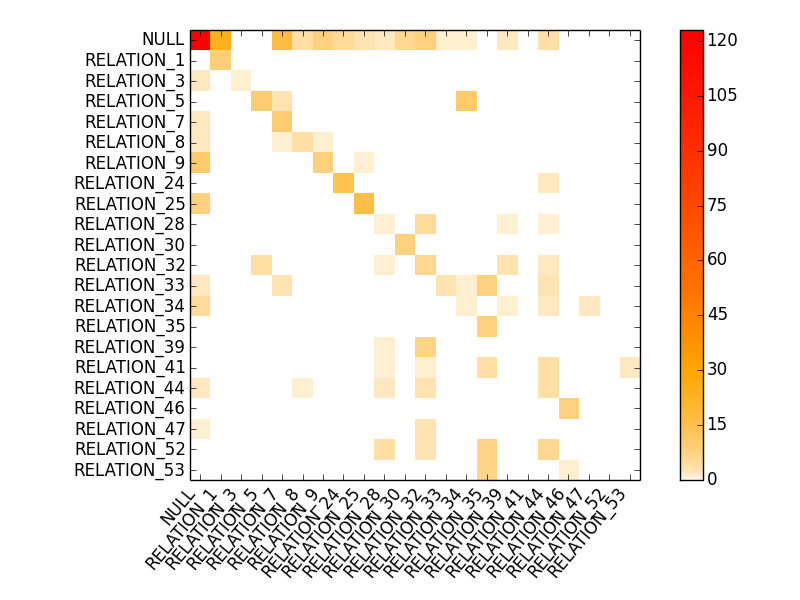
\includegraphics[width=0.5\linewidth]{Figures/Confusion_Matrices/confusionMatrixRelationClassification_noConstraints.png}\hfill
   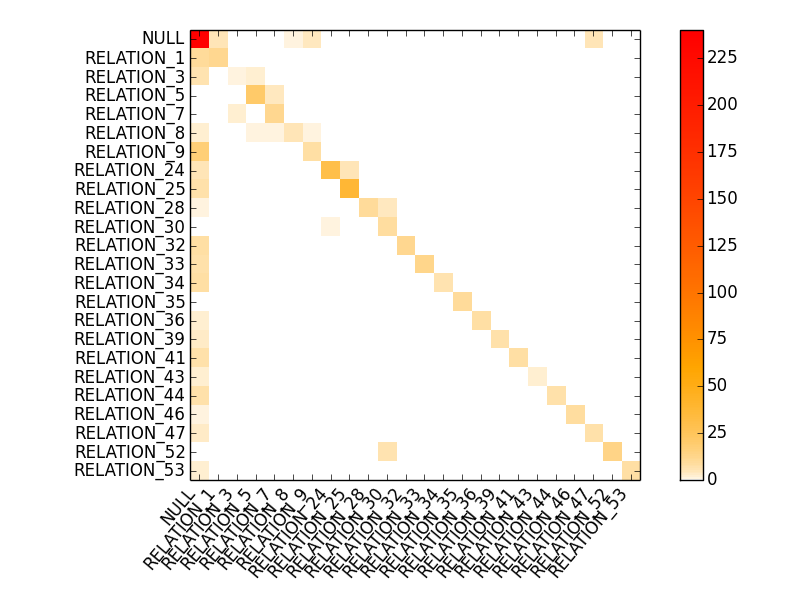
\includegraphics[width=0.5\linewidth]{Figures/Confusion_Matrices/confusionMatrixRelationClassification_constraints.png}
   \caption{\label{relationConfusion} Confusion matrices of relation classification using dependency bigrams features without constraints (left) and with constraints (right)}
\end{figure}

We made a second experiment to show the impact of the quality of the syntactic information that is classified. We saw that our relation classification models classify syntactic paths that are obtained from sentences with syntactic parsers. In this experiment, we use the same relation classification model (SVM model with constraints, using either dependencies unigrams or bigrams, but not words) and the same training dataset, but we use two different syntactic parsers to obtain the syntactic paths from which we extract the features to classify (see Table~\ref{impactSyntaxRelationClassification}).

\begin{table}[!ht]
\center
\begin{tabular}{c||c|c}
	Model & Micro F1 & Macro F1 \\
	\hline
	\hline
	SVM Model & & \\
	with constraints, dependency unigrams & 0.767 & 0.789 \\
	(\textit{Parsey McParseface} Parser) & & \\ \hline
	SVM Model & & \\
	with constraints, dependency bigrams & \textbf{0.792} & \textbf{0.791} \\
	(\textit{Parsey McParseface} Parser) & & \\ \hline
	SVM Model & & \\
	with constraints, dependency unigrams & 0.731 & 0.774 \\
	(\textit{Stanford} Parser) & & \\ \hline
	SVM Model & & \\
	with constraints, dependency bigrams & 0.774 & 0.784 \\
	(\textit{Stanford} Parser) & & \\ \hline
\end{tabular}
\caption{\label{impactSyntaxRelationClassification} Impact of the syntactic information quality on Relation Classification performance}
\end{table}

The two parsers we use are the Stanford Parser \cite{chen2014fast} and the Parsey McParseface Parser \cite{andor2016globally}; the last one have been shown to achieve state-of-the-art performance on the syntactic parsing task.\\
As a result, we observe a significant difference in the performance of the relation classification model, with better performance when using the Parsey McParseface parser to obtain the syntactic paths. This is mainly due to the fact that even a small difference in the syntactic tree of a sentence can lead to big changes in the syntactic paths and make them more difficult to classify correctly with our relation classification models. Therefore, using a syntactic parser that avoid mistakes has a significant positive impact on the relation classification model's performance.

\subsubsection{Conclusion on Relation classification}

As a conclusion on relation classification, we have shown that:
\begin{itemize}
\item A dependency embedding model can be trained from the extracted corpus (after parsing it with a syntactic parser) and allows to classify syntactic paths.
\item Using the ontology's constraints increases performance and speed up the training.
\item Using dependency bigrams instead of unigrams, and then taking into account the order of the dependencies in the syntactic path slightly increases performance.
\item Using both words and dependencies from the paths to classify decreases performance, which shows that we must re-think the way we are using the word information in the path classification.
\item The quality of the syntactic information that we classify in the Relation classification step has a significant impact on performance.
\end{itemize}

\subsection{Crowd-Sourcing}

We saw in the previous sections that working with low resource and small training datasets implies a low recall in the classifications. If we have been able to generate automatically a lot of instances samples to train the instance classification models by using the anchors of the websites we used to extract knowledge about Minecraft, we do not dispose of such a way to generate easily and cheaply training samples for the relation classification yet. This results in a quite low recall in the relation classification step of the semantic parsing.
One solution is to use crowd-sourcing to obtain cheap annotations made by non-expert annotators on the web to increase the size of the training dataset for relation classification.
However, annotating relations between two instances in a text is a difficult task that requires knowing the characteristics of each relation class in the ontology. To make non-expert annotators to realize such an annotation, we need to simplify the annotation task.
What we did is that for each relation sample to be annotated, we generated automatically a short list of propositions in natural language (English) that are easy to understand for human annotators. When annotating the relation between two already automatically classified instances, we begin by building the list of all possible relation class that can be used to link these two instances together. These lists are always rather short, between 1 and about 5 candidates, by construction of the ontology. Then, after having shown the sentence to the annotator, we show him, for each possible relation class, an English proposition that asserts that the relation is true in the context of the sentence and ask him to choose the only proposition that is true (the ontology is designed in a way that there is always at most only one relation between two instances). In the case where there is no relation between the couple of instances (this is a negative sample), the annotator has the possibility to answer that none of the propositions is true. We also ask to the annotator to confirm that the instances have been correctly classified before displaying the propositions in order to avoid wrong annotations of the relation, as wrong instances may lead to a wrong list of possible relation candidates. Each sample is annotated by 5 different annotators, and the most reliable answer is added to the training dataset. We obtained 210 distinct relation samples (158 positive examples, and 52 negative examples) for 9 different relation classes.
This crowd-sourcing has been realized with the CrowdFlower platform\footnote{
\href{http://www.crowdflower.com/}{www.crowdflower.com}} (example in Figure~\ref{crowdSourcing}).

\begin{figure}[!ht]
   \centering 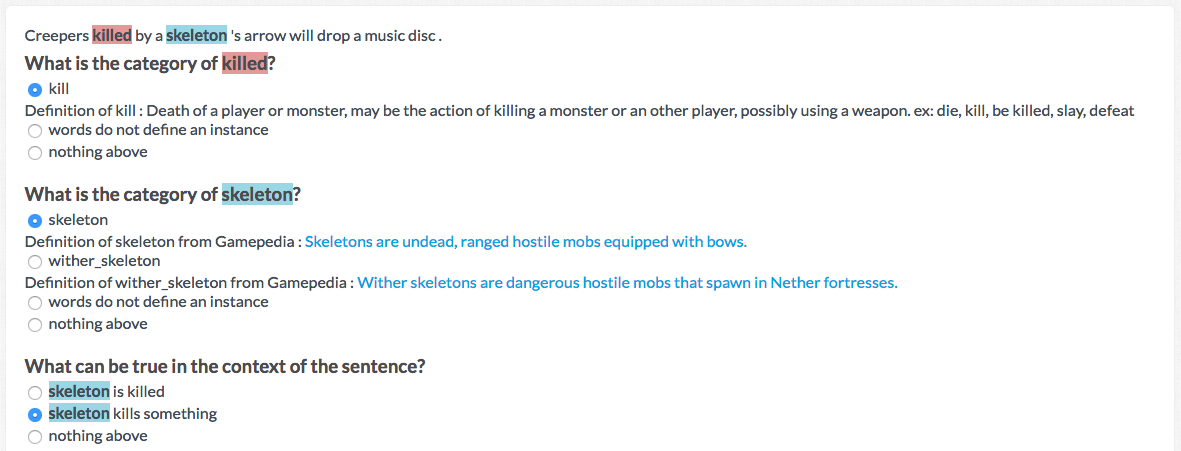
\includegraphics[width=\linewidth]{Figures/Semantic_Parsing/crowdSourcing.png}
   \caption{\label{crowdSourcing} Example of crowd-sourcing annotation with CrowdFlower}
\end{figure}

We evaluated the quality of the annotated data by comparing the performance of the relation classification cross-validation on the crowd-sourcing annotations to the performance of cross-validation on expert annotations (see Table~\ref{crowdSourcingRelationClassification}).

\begin{table}[!ht]
\center
\begin{tabular}{c||c|c}
	Model & Micro F1 & Macro F1 \\
	\hline
	\hline
	SVM Model & & \\
	with constraints, dependency bigrams & \textbf{0.792} & \textbf{0.791} \\
	(expert annotations only) & & \\ \hline
	SVM Model & & \\
	with constraints, dependency bigrams & 0.763 & 0.719 \\
	(crowd-sourcing only) & & \\ \hline
	SVM Model & & \\
	with constraints, dependency bigrams & 0.780 & 0.754 \\
	(expert + crowd-sourcing) & & \\ \hline
\end{tabular}
\caption{\label{crowdSourcingRelationClassification} Relation Classification performance on crowd-sourcing annotations}
\end{table}

If the performance of the cross-validation on crowd-sourcing annotations is slightly below the performance on expert annotations, we can nonetheless conclude that crowd-sourcing can be a good way of increasing the size of the training dataset for relation classification when using the annotating method described before to make the annotation accessible to non-expert annotators.

\newpage
\section{Question Answering}

We dispose of a semantic parser specific to the domain of Minecraft. This semantic parser output knowledge graphs from English sentences, so an interesting issue would now be to study how we can use knowledge graphs to do question answering in Minecraft, and what kind of logical reasoning can be done on knowledge graphs to retrieve answers to difficult questions.\\
This section has for only goal to expose some ideas about a method that can be used to do QA in Minecraft by using the knowledge graphs, and it does not provide any proof or result. Such results could be obtained in a future study, by applying the proposed QA algorithm to the question corpus that have been extracted.

\subsection{Knowledge graphs and question graphs}

We begin with the observation that the semantic parser we built to convert English sentences about Minecraft into knowledge graphs can be as well on the questions. In the short study of this section on question answering, we will divide questions into two categories: question-words questions and yes/no questions that do not contain question words.\\
When applying the semantic parser to a yes/no question (Figure~\ref{yesNoQuestion}), we can see that the question graph is almost identical to the knowledge graph of the corresponding assertion. We will then be able to answer yes/no questions by looking for knowledge graphs similar to the question graphs in the knowledge database. The presence of such a similar knowledge graph giving the answer ``Yes'', and the absence giving the answer ``No''.\\

\begin{figure}[!ht]
   \centering 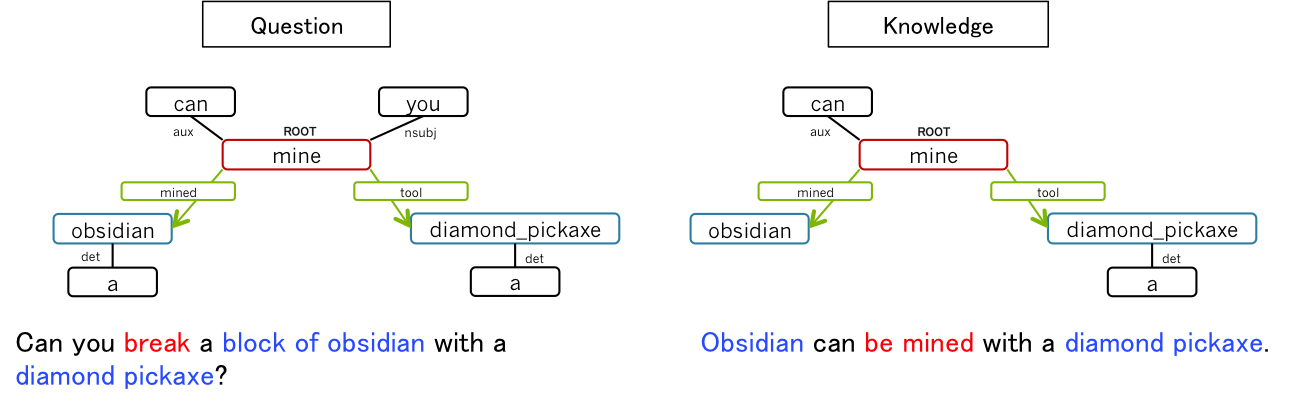
\includegraphics[width=\linewidth]{Figures/Question_Answering/yesNoQuestion.png}
   \caption{\label{yesNoQuestion} Example of yes/no question graph and the corresponding assertion graph}
\end{figure}

When applying the semantic parser to a question-word question (Figure~\ref{qWordQuestion}), we can see that the question graph is similar the knowledge graph containing the answer, with the difference that the question graph has an \textbf{unknown instance node} in the place of the sub-graph that represents the answer. We will then be able to answer question-words questions by looking in the knowledge database for compatible sub-graphs that can be substituted to the unknown instance node.

\begin{figure}[!ht]
   \centering 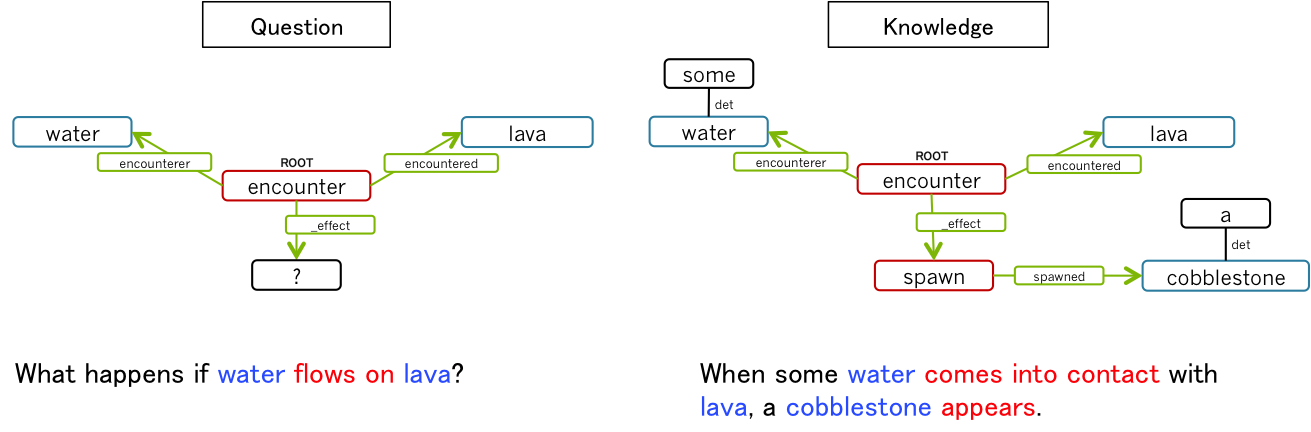
\includegraphics[width=\linewidth]{Figures/Question_Answering/qWordQuestion.png}
   \caption{\label{qWordQuestion} Example of question-word question graph and the knowledge graph of its answer}
\end{figure}

\subsection{QA algorithm}

Several studies have been done on using knowledge graphs to do question answering. Some of them developed methods to retrieve answers from graphs without the need of an ontology, and can be done in open-domain \cite{aghaebrahimianopen,hixon2015learning} because they do not require to convert both question and knowledge to semantic graphs. These algorithms provide an interesting alternative to our method.\\
However, in the case of our study, we are more interesting in the works that make use of both question graphs and knowledge graphs, and developed methods to retrieve answers by graph comparison (common paths and overlaps) between the questions graphs and the knowledge graphs containing candidate answers \cite{molla2005learning,molla2006learning,gomez2014graph}. The algorithm we describe in this section (Algorithm~\ref{QAalgo1},\ref{QAalgo2}) is closely related to these last works.

\begin{algorithm}
\caption{QA algorithm - step 1}\label{QAalgo1}
\begin{algorithmic}
\Procedure{RetrieveCandidates}{$questionGraph$,$knowledgeGraphCollection$}
\State $candidates \gets []$
\If {$questionGraph$ \textbf{is} $yesNoQuestion$}
\ForAll {$knowledgeGraph$ \textbf{in} $knowledgeGraphCollection$}
\If {$questionGraph.root$ \textbf{in} $knowledgeGraph.nodes$}
\State $candidate[0] \gets$ ``Yes''
\State $candidate[1] \gets questionGraph$
\State $candidate[2] \gets knowledgeGraph$
\State $candidates$.append($candidate$)
\EndIf
\EndFor
\ElsIf {$questionGraph$ \textbf{is} $qWordQuestion$}
\State $rootIndex \gets questionGraph.root$
\State $qWordIndex \gets questionGraph$.index($qWord$)
\State $path \gets questionGraph$.path($rootIndex$, $qWordIndex$)
\ForAll {$knowledgeGraph$ \textbf{in} $knowledgeGraphCollection$}
\If {$path$ \textbf{in} $knowledgeGraph.paths$}
\State $candidateNode \gets knowledgeGraph$.paths($path$).$end$
\State $answer \gets candidateNode.subgraph$
\State $candidate[0] \gets answer$
\State $candidate[1] \gets questionGraph$.replace($qWordIndex$,$answer$)
\State $candidate[2] \gets knowledgeGraph$
\State $candidates$.append($candidate$)
\EndIf
\EndFor
\EndIf
\Return $candidates$
\EndProcedure
\end{algorithmic}
\end{algorithm}

\begin{algorithm}
\caption{QA algorithm - step 2}\label{QAalgo2}
\begin{algorithmic}
\Procedure{ValidateAnswers}{$candidates$}
\ForAll {$candidate$ in $candidates$}
\State $answer \gets candidate[0]$
\State $modifiedQuestionGraph \gets candidate[1]$
\State $originKnowledgeGraph \gets candidate[2]$
\If {overlap($modifiedQuestionGraph$,$originKnowledgeGraph$)$ > threshold$}
\State \textbf{Print} ``Answer: '', $answer.text$
\State \textbf{Print} ``Justification: '', $originKnowledgeGraph.text$
\EndIf
\EndFor
\EndProcedure
\end{algorithmic}
\end{algorithm}

For yes/no questions, answering a question consists in comparing the question graph with every knowledge graph in the knowledge database. If any knowledge graph overlaps with the question graph more than a fixed threshold, the answer is ``yes'', otherwise it is ``no''.\\
In the case of question-words questions, retrieving answers is done in two steps. In the first step we retrieve candidates answers. To do this, we consider the path between the root and the unknown instance node in the question graph. Any knowledge graph that contains this path provides a candidate answer, which is the sub-graph at the end of this path. Then, in the second step, for each candidate answer, we replace the unknown instance node by the candidate answer sub-graph, and we compare the modified question graph with the knowledge graph the candidate answer is extracted from. If the overlaps exceeds a fixed threshold, the candidate answer is validated.\\
Note that the obtained answers are semantic graphs, so it is possible to do logical reasoning, by combining different pieces of knowledge from different knowledge graphs to answer. To do this, after having retrieved the answer, we convert it into a new question graph by adding an unknown instance to it and we repeat the algorithm to retrieve answers. An example in given the Appendix~\ref{annexeQA}.

\newpage
\section{Conclusion}

In this work, we presented a study about semantic parsing with very low annotated resource in the domain of the video game Minecraft.
We described the methods used to collect data about the domain and the classification models that we designed to build a semantic parser.
We have shown that such a semantic parser can be performing in the restricted domain if we make good use of the data we created, in particular by using the ontology's characteristics, and that it can be trained with only a few manually annotated resource and can be completed with automatically generated samples or through crowd-sourcing annotations.
We also described a question answering algorithm that allows logical reasoning on the knowledge graphs output by the semantic parser to answer non-factoid questions.\\
Our study brings two main contributions when compared to other works describing methods to build semantic parsers for limited domains \cite{wang2015building}. First, we explored various ways to increase the parsing performance by acting on both the size of the training dataset with several methods (web anchors, crowd-sourcing), and the classification models (integrating ontology in the classification step and extracting relevant features). And secondly, our semantic parser output semantic graphs that are immediately usable by a QA algorithm to answer even difficult questions using logical reasoning.\\
Thus, we believe that our work is then a first step in answering to how to efficiently build a semantic parser with very low resource and use it to do advanced question answering in restricted domains.\\

As future works, we believe that some work should be done to improve the relation classification step of the semantic parsing. Indeed, the recall still has to be reduced, which implies a lot of manual annotations with the current methodology. One interesting problematic could be to answer the question: can we create training data automatically from available resource, as we did with anchors for instance classification? We could for example imagine that we look for typical couples of instances that can only be linked by one possible relation in a natural language corpus to create automatically relations samples.\\
We think that some work should also be done to reduce even more the quantity of manual work needed to build the ontology of the restricted domain. There have been some interesting works on how a system can learn to produce knowledge graphs without any ontology \cite{hixon2015learning} that have shown that the performance are particularly good in restricted domains. Or may even be possible to limit semantic parsing to instance classification and do question answering directly on syntactic trees \cite{gomez2014graph}.
Then, a deeper study should be done on the application of the knowledge graphs produced by semantic parsing on question answering in Minecraft. The algorithm should be improved by inspiring from other studies on graph-based question answering systems \cite{molla2005learning,molla2006learning} and tested on the corpus of questions that has already been collected.\\
Finally, it would be interesting to use our models to train and test a semantic parser and a QA system on other low resource restricted domains \cite{molla2007question} such as technical fields (medical domain, industrial domains, \emph{etc.}), customer services, or other video games.

% acknowledgements
\newpage
\acknowledgements
I would first like to express my gratitude to my supervisor Professor Kentaro Inui from the Graduate School of Information Sciences at Tohoku University. Professor Inui has been of great help, not only for supervising my research, but also for my student life in general. My master thesis in Tohoku University would not have been possible without him.\\
I am also deeply indebted to Research Assistant Professor Ran Tian and Associate Professor Naoaki Okazaki for their continuous guidance over the duration of my research. I would like to thank them for their implication, and for the time they spent giving me the advices and inspiration that oriented my work.\\
I would like to thank Professor Yoshifumi Kitamura and Professor Tetsuo Kinoshita who were involved in the validation of this research project.\\
Furthermore, I would like to thank the people from the Incoming Student Exchange Section and the JASSO scholarship program very deeply for their kindness and their involvment. The JASSO scholarship really allowed me to integrate better in the Japanese society, as I could participate to more events and sometimes travel with friends to discover new beautiful places in Japan.\\
Finally, I would also like to thank all the Inui-Okazaki laboratory members, professors, researchers and students, for their valuable comments and support, and for having created together a very pleasant working environment.

\newpage
% References
\bibliography{references}
\bibliographystyle{unsrt}

\newpage
% Appendix
\appendix

\section{\label{annexeQA}Question Answering: example of logical reasoning on knowledge graphs}

\begin{figure}[!htbp]
   \centering 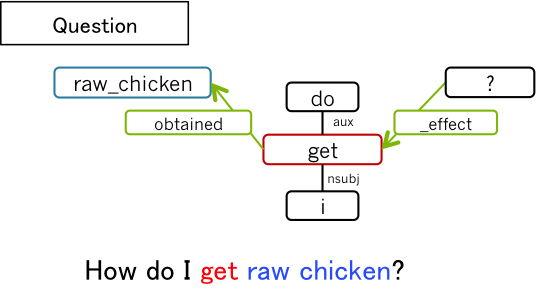
\includegraphics[width=0.6\linewidth]{Figures/Question_Answering/question.png}
   \caption{\label{questionEx} Question graph}
\end{figure}

\begin{figure}[!htbp]
   \centering 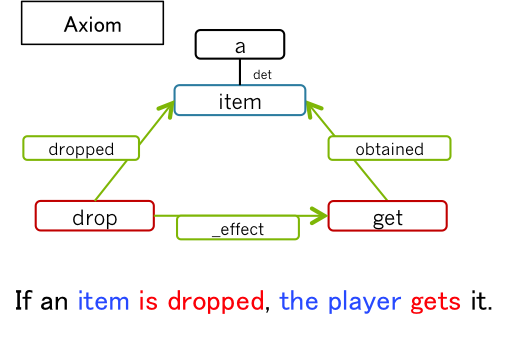
\includegraphics[width=0.6\linewidth]{Figures/Question_Answering/axiom.png}
   \caption{\label{axiomEx} Axiom}
\end{figure}

\begin{figure}[!htbp]
   \centering 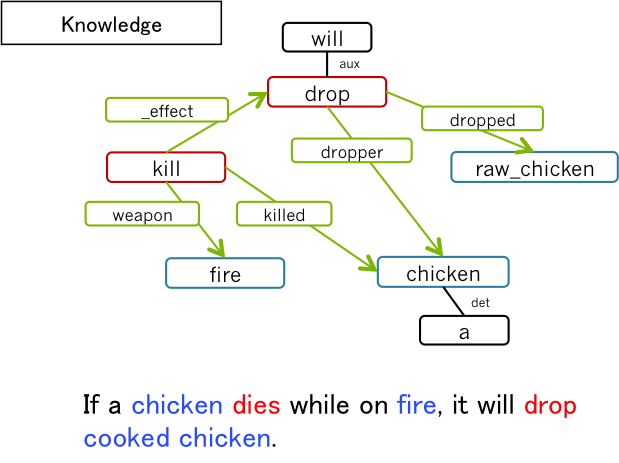
\includegraphics[width=0.6\linewidth]{Figures/Question_Answering/knowledge.png}
   \caption{\label{knowledgeEx} Piece of knowledge}
\end{figure}

\begin{figure}[!htbp]
   \centering 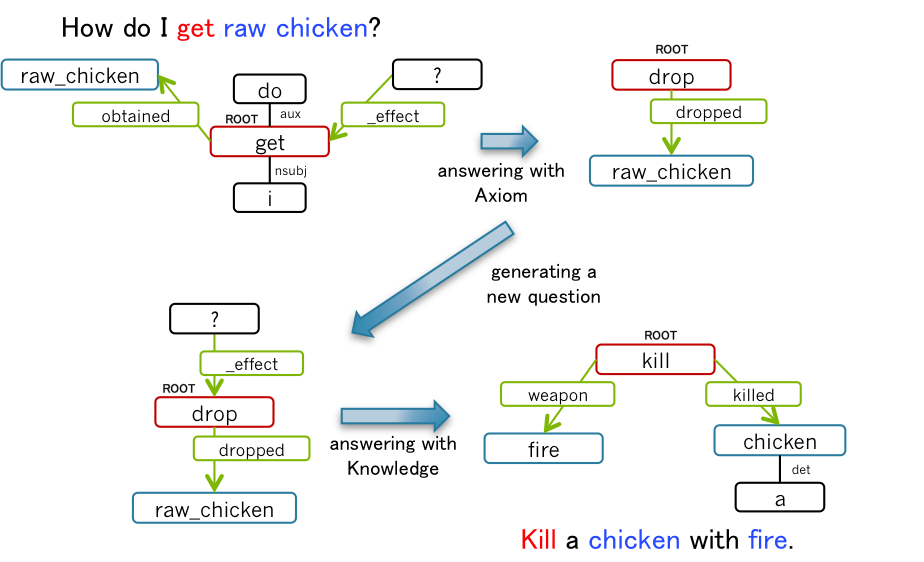
\includegraphics[width=0.9\linewidth]{Figures/Question_Answering/answer.png}
   \caption{\label{answerEx} Logical reasoning to retrieve the answer}
\end{figure}

\newpage
% Publications List
% For English
% 査読あり:refereed
% 査読なし:domestic
\section*{List of Publications}
%\subsection*{Awards}
%\subsection*{Journal Papers}
\subsection*{International Conferences Papers}

\begin{itemize}
\item Corentin Dumont, Ran Tian, and Kentaro Inui. question answering with
logic specific to video games. Language Resources and Evaluation Conference, 2016.
\end{itemize}

\subsection*{Other Publications}

\begin{itemize}
\item Corentin Dumont, Ran Tian, and Kentaro Inui. An ontology for question-
answering on minecraft. The Association for Natural Language Processing, 2016.
\end{itemize}

% For Japanese
%\section*{発表文献一覧}
%\subsection*{受賞一覧}
%\subsection*{学術論文誌}
%\subsection*{国際会議論文}
%\subsection*{国内会議・研究会論文}

\end{document}